\documentclass[11pt,twoside]{article}

\usepackage[margin=1in]{geometry}
\usepackage{amsmath,amssymb,amsthm,mathtools}
\usepackage{array,booktabs}
\usepackage[inline,shortlabels]{enumitem}
\usepackage{xcolor}
\usepackage{../misc_files/course-definition-boxes}
\usepackage{microtype}
\usepackage{tikz}
\usetikzlibrary{arrows.meta,positioning,calc,fit,backgrounds}
\usepackage{listings}
\usepackage{../exercises/course-exercises}

% Revision date: maintained by scripts/build_lecture_notes.py.
\newcommand{\lecturerevised}{2026-11-18 11:06 UTC-06:00}
\usepackage{eso-pic}
\AddToShipoutPictureBG{%
  \AtPageLowerLeft{%
    \put(\LenToUnit{0.5\paperwidth},\LenToUnit{0.5in}){%
      \makebox(0,0){\normalfont\footnotesize\color{black!60}Last revised: \lecturerevised}%
    }%
  }%
}
\usepackage[square,authoryear]{natbib}
\usepackage[colorlinks=true,linkcolor=blue!60!black,
  urlcolor=blue!60!black,citecolor=blue!60!black]{hyperref}
\usepackage[nameinlink,capitalize]{cleveref}
\newcommand{\appendixref}[1]{\hyperref[#1]{Appendix~\ref*{#1}}}
\usepackage{enotez}
\DeclareInstance{enotez-list}{lecture}{list}{format=\normalsize,number={#1.}}
\setenotez{list-name=Endnotes,list-style=lecture,backref=true}
\crefname{endnote}{Endnote}{Endnotes}
\Crefname{endnote}{Endnote}{Endnotes}

\definecolor{courseblue}{HTML}{17365D}
\definecolor{lightblue}{HTML}{E8EFF7}
\definecolor{memorygreen}{HTML}{21664D}
\definecolor{lightgreen}{HTML}{EAF4EF}
\definecolor{signalred}{HTML}{A53232}
\newcommand{\E}{\mathbb E}
\newcommand{\I}{\mathbb I}
\renewcommand{\P}{\mathbb P}
\newcommand{\R}{\mathbb R}
\newcommand{\KL}{D}
\newcommand{\TV}{\mathrm{TV}}
\makeatletter
\@for\@letter:=A,B,C,D,E,F,G,H,I,J,K,L,M,N,O,P,Q,R,S,T,U,V,W,X,Y,Z\do{%
  \expandafter\edef\csname c\@letter\endcsname{\noexpand\mathcal{\@letter}}}
\makeatother
\newcommand{\lecturenumber}{16}
\newcommand{\eos}{\mathtt{EOS}}
\newcommand{\sep}{\mathtt{SEP}}
\newcommand{\enc}{\operatorname{enc}}
\newcommand{\tab}{\operatorname{tab}}
\newcommand{\sat}{\operatorname{sat}}

\newtheorem{theorem}{Theorem}[section]
\newtheorem{proposition}[theorem]{Proposition}
\newtheorem{corollary}[theorem]{Corollary}
\newtheorem{lemma}[theorem]{Lemma}
\theoremstyle{definition}
\newtheorem{definition}[theorem]{Definition}
\newtheorem{example}[theorem]{Example}
\theoremstyle{remark}
\newtheorem{remark}[theorem]{Remark}
\crefname{exercise}{Exercise}{Exercises}
\Crefname{exercise}{Exercise}{Exercises}

\renewcommand{\thepage}{16--\arabic{page}}
\renewcommand{\thesection}{16.\arabic{section}}
\renewcommand{\theequation}{16.\arabic{equation}}
\pagestyle{myheadings}
\markboth{Lecture 16: Runtime systems and long computation}
{Lecture 16: Runtime systems and long computation}
\hypersetup{pdftitle={Lecture 16: Runtime systems and long computation},
 pdfauthor={Csaba Szepesvari}}
\tikzset{module/.style={draw=courseblue,thick,rounded corners=2pt,
 fill=lightblue,align=center,minimum height=10mm},
 memory/.style={draw=memorygreen,thick,fill=lightgreen,align=center},
 flow/.style={-{Latex[length=2mm]},thick},
 info/.style={font=\small,align=center}}
\lstset{basicstyle=\small\ttfamily,columns=fullflexible,
 keepspaces=true,frame=single,framerule=0.3pt,
 xleftmargin=0.5em,xrightmargin=0.5em,aboveskip=1em,belowskip=1em}

\begin{document}
\begin{center}
\fcolorbox{courseblue}{white}{%
\begin{minipage}{0.92\textwidth}
\vspace{1mm}
\textbf{CMPUT 654: Mathematical Foundations of Modern AI Systems}
\hfill Fall 2026
\vspace{3mm}
\begin{center}
{\Large\bfseries Lecture 16: Runtime systems and long computation}
\vspace{1mm}

October 27, 2026
\end{center}
\vspace{2mm}
\textit{Lecturer: Csaba Szepesv\'ari}\hfill
\textit{Notes prepared by: Csaba Szepesv\'ari}
\vspace{1mm}
\end{minipage}}
\end{center}

Can a language model and a simple runtime execute arbitrary computations?
\href{lecture14.pdf}{Lecture 14} gave a finite neural controller an external
tape and a specially encoded program. Here we ask how generic execution and
memory operations can extend a given model's reliable performance on short
computations to larger tasks. The intended application is a model that
interprets instructions, including natural language, while generic software
supplies execution and memory. The answer depends on the information and
operations supplied by the runtime; extra generation steps alone need not
increase retained state.

\noindent\textbf{Scope and reading guide.}
\Crefrange{sec:interfaces}{sec:stack} follow the classroom sequence through
analysis/synthesis and the limitation of one stack. Precise representation
bounds and several formal statements extend that discussion. Later main
sections develop saved references, read-only recursion, caching, and data
construction. The constraint-combination example, queue construction, and
quantitative transformer simulations are optional; the tree-summary result
is deferred to \appendixref{app:trees}.
The main development concerns exact computation under a stated local
competence assumption. The prerequisites are functions, strings, induction,
and Lecture~14's finite-controller account of Turing machines; complexity
classes are defined where needed.

\section{The model and its runtime}
\label{sec:interfaces}

A model call and an AI system have different interfaces. We assume
deterministic computation throughout: all decoding and control choices
follow fixed rules. Let $\Sigma$ be a
finite token alphabet containing both ordinary tokens and distinguished
\emph{control tokens}, including $\eos,\sep\in\Sigma$. Ordinary data
strings use a subalphabet $\Delta\subset\Sigma$ that excludes these two
tokens. Literal occurrences of reserved tokens can be escaped when data
are encoded. Write $\Sigma^*$ for the
set of finite token strings. With a fixed deterministic decoding rule, a
next-token model has the form
\begin{equation}
 p:\Sigma^*\longrightarrow\Sigma.
 \label{eq:token-model}
\end{equation}
We call $p$ the \emph{next-token rule}. Before deterministic decoding, a
probabilistic model gives a \emph{next-token kernel}
$\pi(\cdot\mid h)$, a probability distribution on $\Sigma$ for each prefix
$h$. The rule in \eqref{eq:token-model} selects one token from that
distribution using a fixed decoding and tie-breaking convention.
The model returns a token; the runtime gives a control token its operational
meaning. The minimum runtime below treats $\eos$ as the instruction to end
the current model call. Richer runtimes can assign operations to further
control tokens, such as marking a tool request or a subproblem return.
To turn $p$ into a string-producing model call, software must retain the
prefix, append generated tokens, and check for termination. We use
\begin{equation}
 f:\Sigma^*\rightharpoonup\Sigma^*
 \label{eq:call-model}
\end{equation}
for this \emph{model-call interface}. The partial arrow allows a call that
does not terminate. All trusted calls below terminate.
\Cref{sec:generation-runtime} constructs $f$ explicitly from $p$ and the
software that runs its generation loop.

\emph{Runtime system} is an established term from programming-language
implementation for software that supports a program's execution. The name
reflects the distinction between \emph{compile time}, when a program is
translated for execution, and \emph{run time}, when the program executes.
Runtime services include maintaining call stacks, allocating and reclaiming
memory, handling exceptions, and providing input/output. Java's virtual
machine and .NET's
Common Language Runtime are familiar examples. In an AI system, a runtime
prepares inputs for models and tools, stores their results, and determines
the next execution step. We represent this software
by an algorithm $R$; with access to model $f$, it computes a partial
function $R^f$ from system inputs to system outputs. The superscript records
access to $f$; the runtime's memory and control operations must be stated
separately.

In LLM engineering, the surrounding software is often called an
\emph{agent harness}. In these notes, \emph{runtime system} and
\emph{agent harness} denote the same surrounding software; we use the
established term \emph{runtime system} throughout. Such software can supply
prompts, tool access, context
management, persistent storage, and stopping rules. For example,
Claude Code supplies an execution loop with file and command-line tools;
OpenHands coordinates model calls, tool execution, and conversation
context; and Deep Agents supplies planning tools, a filesystem interface,
and calls to subagents.

\begin{figure}[htbp]
\centering
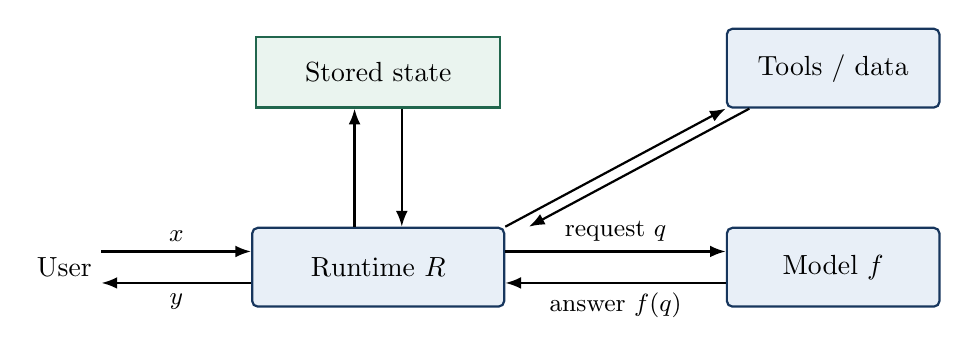
\begin{tikzpicture}[node distance=19mm]
\node (user) {User};
\node[module,minimum width=32mm,right=of user] (rt) {Runtime $R$};
\node[module,minimum width=27mm,right=28mm of rt] (model) {Model $f$};
\node[memory,minimum width=31mm,minimum height=9mm,above=15mm of rt] (mem) {Stored state};
\node[module,minimum width=27mm,above=15mm of model] (tools) {Tools / data};
\draw[flow] ([yshift=2mm]user.east)--node[above,info]{$x$}([yshift=2mm]rt.west);
\draw[flow] ([yshift=-2mm]rt.west)--node[below,info]{$y$}([yshift=-2mm]user.east);
\draw[flow] ([yshift=2mm]rt.east)--node[above,info]{request $q$}([yshift=2mm]model.west);
\draw[flow] ([yshift=-2mm]model.west)--node[below,info]{answer $f(q)$}([yshift=-2mm]rt.east);
\draw[flow] ([xshift=-3mm]rt.north)--([xshift=-3mm]mem.south);
\draw[flow] ([xshift=3mm]mem.south)--([xshift=3mm]rt.north);
\draw[flow] (rt.north east)--(tools.south west);
\draw[flow] ([xshift=3mm]tools.south west)--([xshift=3mm]rt.north east);
\end{tikzpicture}
\caption{A task runtime with stored state and tools. The minimal task
runtime simply forwards $x$ to $f$ and returns $f(x)$. Richer runtimes
determine which information reaches each call and what remains available
afterward; the results below state which resources are permitted.}
\label{fig:system}
\end{figure}

\subsection{The minimum autoregressive runtime: defining \texorpdfstring{$f$}{f} from \texorpdfstring{$p$}{p}}
\label{sec:generation-runtime}

The first universality question needs no task-specific runtime: how much
can a model do when software only runs its generation loop? Here
\emph{computational universality} means the ability to execute every
computable program under a suitable input encoding. We will also consider
the stronger representation question of realizing every string-to-string
map, including maps that are not computable.

Let $G$ be the generation runtime that repeatedly invokes $p$ and appends
each generated token to its input. Given a request $x$, initialize
$h_0=x\sep$. The separator marks where the supplied request ends and the
generated answer begins. At step $t$, compute $a_t=p(h_t)$. If $a_t=\eos$, stop;
otherwise set
\begin{equation}
 h_{t+1}=h_ta_t.
 \label{eq:append}
\end{equation}
If $\tau$ is the first step with $a_\tau=\eos$, define
\begin{equation}
 f(x)=G^p(x)=a_0\cdots a_{\tau-1}.
 \label{eq:generated-call}
\end{equation}
The output excludes both the supplied prefix and the stop symbol. If
$\tau=0$, the output is the empty string; if no stop symbol occurs,
$f(x)$ is undefined. Thus a next-token computation $p$ and a generation
runtime $G$ together implement the model-call function $f$.

The simplest system returns $f(x)$ directly: the generation runtime $G$
already supplies its execution and memory operations. An additional task
runtime is optional. In the notation $R^f$, the minimal choice $R_0$ merely
passes $x$ to $f$ and returns the answer, so $R_0^f(x)=f(x)$.

\Needspace{6\baselineskip}
A richer task runtime $R$ can make several calls to $f$, retain their
answers, and use tools between calls. When both levels are present, they satisfy
\begin{equation}
 f=G^p,\qquad R^f=R^{G^p}.
 \label{eq:nested-runtimes}
\end{equation}
\Needspace{5\baselineskip}
An $\eos$ token stops $G$ and returns its answer to the caller. If the caller
is a task runtime $R$, that runtime may then make another model call.
The distinction is between individual token steps within one call and
model calls within a larger task. Calling $f$ may already involve many
steps of $p$; a bound on a call's input length is different from a bound
on its generated output.

\begin{figure}[!htb]
\centering
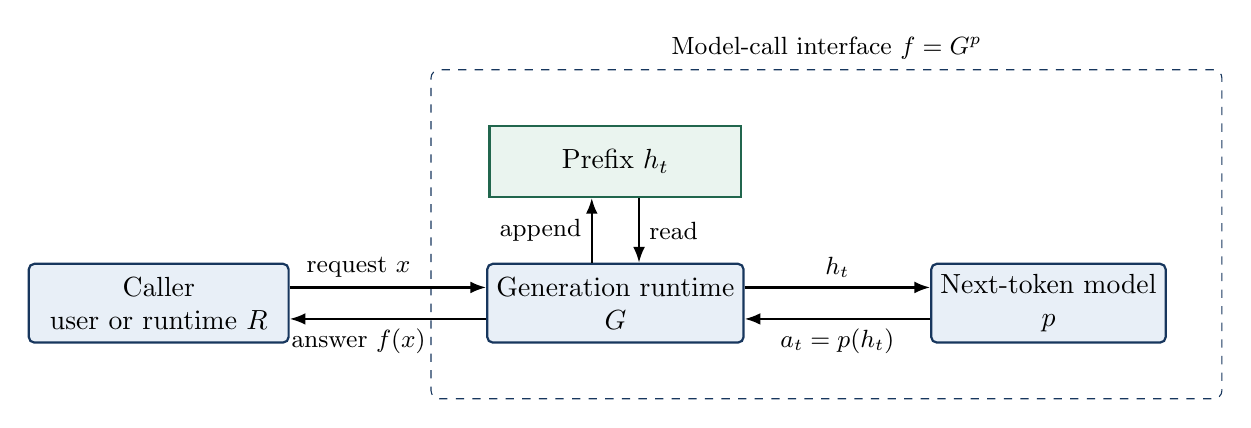
\begin{tikzpicture}
\node[module,minimum width=33mm] (outer) at (0,0) {Caller\\user or runtime $R$};
\node[module,minimum width=32mm] (gen) at (5.8,0) {Generation runtime\\$G$};
\node[module,minimum width=27mm] (next) at (11.3,0) {Next-token model\\$p$};
\node[memory,minimum width=32mm,minimum height=9mm] (prefix) at (5.8,1.8)
 {Prefix $h_t$};
\node[draw=courseblue,dashed,rounded corners=3pt,
 fit=(gen)(next)(prefix),inner sep=7mm,
 label={[font=\small]above:Model-call interface $f=G^p$}] (call) {};
\draw[flow] ([yshift=2mm]outer.east)--node[above,info,pos=0.35]{request $x$}
 ([yshift=2mm]gen.west);
\draw[flow] ([yshift=-2mm]gen.west)--node[below,info,pos=0.65]{answer $f(x)$}
 ([yshift=-2mm]outer.east);
\draw[flow] ([yshift=2mm]gen.east)--node[above,info]{$h_t$}
 ([yshift=2mm]next.west);
\draw[flow] ([yshift=-2mm]next.west)--node[below,info]{$a_t=p(h_t)$}
 ([yshift=-2mm]gen.east);
\draw[flow] ([xshift=-3mm]gen.north)--node[left,info]{append}
 ([xshift=-3mm]prefix.south);
\draw[flow] ([xshift=3mm]prefix.south)--node[right,info]{read}
 ([xshift=3mm]gen.north);
\end{tikzpicture}
\caption{A model call has its own runtime. A user can call $f$ directly;
an additional task runtime $R$ is optional. Inside the interface $f=G^p$,
$G$ stores a prefix, invokes $p$, appends tokens, and stops at $\mathtt{EOS}$.}
\label{fig:nested-runtimes}
\end{figure}

\subsection{Chain-of-thought prompting and answer extraction}
\label{sec:cot}

A familiar variation asks the model to generate intermediate reasoning
before its answer, then returns only the answer. The runtime performs two
small operations around the generation loop: it adds prompting instructions
and extracts the final answer. We formalize one such \emph{chain-of-thought
protocol}.

Reserve a further control token $\mathtt{FINAL}\in\Sigma$ and write
$\Omega=\Sigma\setminus\{\mathtt{FINAL},\eos\}$. The prompt-preparation
map $J:\Sigma^*\to\Sigma^*$ has the form $J(x)=j_{\mathrm{pre}}xj_{\mathrm{post}}$
for fixed instruction strings $j_{\mathrm{pre}},j_{\mathrm{post}}\in\Sigma^*$.
Those instructions ask the model to work through intermediate steps and
produce the format
\[
 r\,\mathtt{FINAL}\,y,\qquad r,y\in\Omega^*.
\]
Here $r$ is the generated reasoning and $y$ is the final answer. The
generation runtime stops at $\eos$ as before. Define the extraction map
$E:\Sigma^*\rightharpoonup\Omega^*$ by
\begin{equation}
 E(r\,\mathtt{FINAL}\,y)=y\quad(r,y\in\Omega^*),\qquad
 R_{\mathrm{CoT}}^f=E\circ f\circ J=E\circ G^p\circ J.
 \label{eq:cot-runtime}
\end{equation}
The marker must occur exactly once; other generated strings are formatting
failures for this protocol. Literal occurrences can be escaped. Prompting
requests the format but does not guarantee that the model follows it.

\begin{figure}[htbp]
\centering
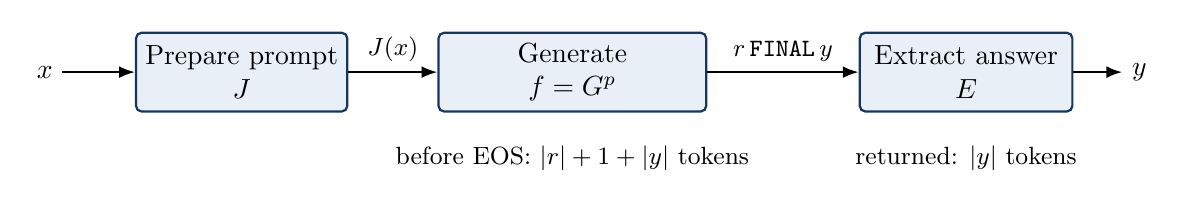
\begin{tikzpicture}[x=10mm,y=10mm]
\node (x) at (-2.5,0) {$x$};
\node[module,minimum width=25mm] (prep) at (0,0) {Prepare prompt\\$J$};
\node[module,minimum width=34mm] (gen) at (4.2,0) {Generate\\$f=G^p$};
\node[module,minimum width=27mm] (extract) at (9.2,0) {Extract answer\\$E$};
\node (y) at (11.4,0) {$y$};
\draw[flow] (x)--(prep);
\draw[flow] (prep)--node[above,info]{$J(x)$}(gen);
\draw[flow] (gen)--node[above,info]{$r\,\mathtt{FINAL}\,y$}(extract);
\draw[flow] (extract)--(y);
\node[info] at (4.2,-1.1) {before EOS: $|r|+1+|y|$ tokens};
\node[info] at (9.2,-1.1) {returned: $|y|$ tokens};
\end{tikzpicture}
\caption{A chain-of-thought protocol adds prompt preparation and final-answer
extraction around one model call. During generation, the reasoning is part
of the history available under the runtime's context policy. Extraction
omits that reasoning from the returned response.}
\label{fig:cot-runtime}
\end{figure}

The two output lengths are different resources. On a correctly formatted
run,
\begin{equation}
 |f(J(x))|=|r|+1+|y|,\qquad |R_{\mathrm{CoT}}^f(x)|=|y|.
 \label{eq:cot-lengths}
\end{equation}
Thus a short returned answer can follow a long generated computation.
The extraction step does not reclaim context during generation; which
earlier tokens remain accessible is still determined by the context policy.

\paragraph{Learning a repeated transition.}
A controlled empirical example compares two ways to learn finite-state
dynamics. Let \(Q\) be a finite state set and \(\cU\) a finite input alphabet,
with disjoint one-token encodings in the model's vocabulary \(\Sigma\).
We suppress those encodings in the displayed sequence below.
For an input sequence \(u_{1:T}\), a transition rule
\(\delta:Q\times\cU\to Q\), and a fixed initial state \(s_0\in Q\), the
target states satisfy \(s_t=\delta(s_{t-1},u_t)\).
Lecture~14 shows that a logarithmic-depth transformer can represent the trajectory
by parallel composition. Alternatively, a \emph{scratchpad} records
intermediate states in the sequence. Training can supply interleaved inputs
and correct states; at evaluation, the runtime supplies each next input
and appends the model's predicted state:
\[
 u_1,\widehat s_1,u_2,\widehat s_2,\ldots,u_T,\widehat s_T.
\]
Set \(\widehat s_0=s_0\). The model can then predict \(\widehat s_t\)
using \(u_t\) and \(\widehat s_{t-1}\). The runtime performs \(T\) successive
state predictions, allowing the same local transition rule to be reused
at every step.

In experiments on finite-state tasks, shallow transformers learned accurate
predictions on the training distribution but could fail when input
frequencies or sequence lengths changed. Scratchpad training combined with
an attention bias toward recent positions improved generalization in the
tested settings. The scratchpad alone leaves the model free to ignore
earlier state predictions and use a parallel computation.
The intervention changes training and attention as well as execution;
the evidence does not establish that requesting extra reasoning from an
unchanged model produces the same benefit. The bibliographical notes give
the experimental source and scope.

\subsection{Resources that must be distinguished}

Long tasks can exceed a single call in several different ways. We record
input length $|x|$, output length $|y|$, number of model calls, the maximum
input and output lengths of a call, and the maximum stored state. Model
size and numerical precision are separate parameters. A short program may
run for a long time and allocate substantial memory; a long document may
require only a one-bit final decision.

An \emph{output stream} supports appending symbols without reading previous
output. Such a stream permits arbitrarily long total answers while individual
emissions remain bounded. If later steps can reread or edit the output,
the output has become an additional memory device. We keep that distinction
in every machine model below.

\section{What generation alone can compute}
\label{sec:autoregression}

Generation separates a string transformation into next-token decisions.
Whether those decisions can be represented by a finite transformer is an
additional constraint. We first remove that constraint, then impose an
architecture, numerical precision, and a context bound in turn.

\subsection{An unrestricted next-token rule}

If no restriction is placed on $p$, the generation format can express
every transformation of finite data strings.

\begin{proposition}[Every string map has a next-token representation]
\label{prop:arbitrary-rule}
For every function $F:\Delta^*\to\Delta^*$, there exists a rule
$p:\Sigma^*\to\Sigma$ such that the generation runtime initialized with
$h_0=x\sep$ satisfies
\begin{equation}
 G^p(x)=F(x)\qquad(x\in\Delta^*).
 \label{eq:arbitrary-rule}
\end{equation}
No computability assumption on $F$ or $p$ is required.
\end{proposition}

\Cref{ex:l16-autoregressive-representation} asks you to construct $p$ and
prove the proposition. The separator is part of the interface: the rule
must distinguish supplied input from generated output. The result is a
representation statement. All the difficulty of the task may reside in
the rule $p$.

\subsection{What changes when the rule must be a neural network?}

A transformer computes its next-token rule through a particular finite
architecture: token and positional representations, a fixed number of
attention heads and layers, feed-forward blocks, and an output decoder.
For a target rule $p$, the question is whether some parameter choice
$\theta$ gives
\begin{equation}
 T_\theta(h)=p(h)\qquad\text{for every relevant prefix }h.
 \label{eq:represent-rule}
\end{equation}
The quantifiers matter. Choosing a larger network for each context bound
is different from using one fixed network at every input length.

Numerical assumptions also matter. In an \emph{exact-real model}, weights
and activations can be arbitrary real numbers and arithmetic is exact.
In a \emph{fixed-precision model}, every stored numerical value belongs to
a specified finite set, with fixed rules for rounding and overflow. The
latter includes idealizations of floating-point and fixed-point hardware.

Exact real values can contain infinitely much task-specific information.
Recurrent networks show how repeated computation can access that information.

\begin{theorem}[Arbitrary languages with exact-real recurrence; stated without proof]
\label{thm:real-rnn}
There is a fixed finite recurrent-network architecture with saturated-linear
activation $\sigma(z)=\min\{1,\max\{0,z\}\}$ such that, for every
language $L\subseteq\{0,1\}^*$, a choice of real weights makes the network
halt with the answer $\I\{x\in L\}$ on every finite input $x$.
The weights and recurrent state use exact real arithmetic, and the number
of recurrent steps is not bounded by the architecture's size.
\end{theorem}

The information source can be understood by enumerating binary strings
$x_1,x_2,\ldots$ and encoding their membership bits in one real number,
for example
\begin{equation}
 r_L=\sum_{j\geq1}\bigl(1+2\I\{x_j\in L\}\bigr)4^{-j}.
 \label{eq:real-advice}
\end{equation}
Repeated state updates can extract successively later digits. The
network construction implements the required access and control;
the displayed encoding explains where the answers are stored. Choosing
an uncomputable $L$ gives computation beyond Turing computability.
Arbitrary finite-string outputs can also be obtained by encoding the
graph of a function and recurrently searching for its output.\endnote{From
languages to string maps. For a total $F$, encode
$L_F=\{\operatorname{enc}(x,y):F(x)=y\}$ in an exact-real language recognizer.
A finite recurrent controller can enumerate candidate $y$ in length-lexicographic
order and use the recognizer until the correct $y$ is found. Every run
terminates, but no computable uniform time or output-length bound follows.
This is a consequence of exact-real recurrent control, not a claim about
one transformer forward pass.}\label{en:string-output}

An arbitrarily small change in $r_L$ can change answers encoded far enough
out in its expansion. Consequently, the theorem does not provide a
uniform tolerance to fixed nonzero errors in storage or arithmetic.
The \emph{physical Church--Turing thesis} asserts, in one common form,
that physically realizable computations are Turing-computable. It is a
claim about physical realizability, not a mathematical prohibition on
the exact-real model. For practical systems, finite precision and noise
make the resources hidden in an exact real number essential to disclose.

\subsection{A limitation for a single exact-real transformer pass}

The RNN result uses repeated state updates. A transformer forward pass has
fixed depth, although the number of token positions can grow. Feed-forward
structure alone does not establish a limitation; the permitted operations
must be specified. For standard softmax and ReLU operations, there is now
a precise limitation. This result supplements the discussion in class.

A binary function family \emph{shatters} a set of inputs if it realizes
every assignment of zero and one to those inputs. Its \emph{VC dimension}
is the largest size of a shattered set.

\begin{theorem}[Exact-real weights do not remove fixed-architecture limits; stated without proof]
\label{thm:real-transformer}
Fix a transformer's depth, head count, hidden and feed-forward dimensions,
and an additive positional encoding rule independent of its trainable
parameters. Use softmax attention, ReLU feed-forward blocks, residual
connections, and optionally layer normalization with a fixed positive
stabilizer. Causal or unmasked attention is allowed. Let $\cH_t$ be the
binary decisions obtainable on length-$t$ inputs by varying the real
parameters, with exact arithmetic, in one forward pass. For a constant
$C$ depending on the fixed architecture,
\begin{equation}
 \operatorname{VCdim}(\cH_t)\leq Ct^4.
 \label{eq:real-vc}
\end{equation}
In particular, if $2^t>Ct^4$, some Boolean map on $\{0,1\}^t$ cannot
be represented by that architecture.
\end{theorem}

The final conclusion follows because representing every Boolean map would
shatter all $2^t$ binary inputs. The theorem concerns one fixed architecture
and one pass. It permits a larger architecture when $t$ grows and does not
bound the power of repeated autoregressive generation. The real-weight
RNN and transformer statements therefore compare different computational
resources, even before numerical precision is restricted.
The limitation is about representing \emph{every} task. Even one exact-real
transformer pass can compute some noncomputable tasks.\endnote{A
noncomputable threshold. Fix a noncomputable real $\alpha\in(0,1)$.
Uniform attention can compute the fraction of ones in a nonempty binary
string $w$, and a real-weight output comparison can decide
$\#_1(w)/|w|<\alpha$. A decision algorithm for all such strings would
permit rational comparisons and hence arbitrary-precision computation of
$\alpha$. Thus a single noncomputable weight can already make this
language noncomputable; the VC-dimension bound concerns the larger claim
of representing all languages with one fixed architecture.}

\subsection{Finite descriptions: a counting obstruction}

At fixed precision, a simpler argument applies to any finitely encoded
architecture. Let $\cF_b$ be the next-token rules obtainable from a fixed
$b$-bit parameter storage state, with the architecture and numerical
operations fixed. Thus
\begin{equation}
 |\cF_b|\leq 2^b.
 \label{eq:description-count}
\end{equation}

\begin{proposition}[Description bits required to represent all finite tasks]
\label{prop:description-bits}
Let $D$ contain $N$ inputs and let the output alphabet contain $q\geq2$
symbols. A family described by $b$ bits represents at most $2^b$ of the
$q^N$ maps $D\to[q]$. Representing every such map therefore requires
\begin{equation}
 b\geq N\log_2 q.
 \label{eq:count-obstruction}
\end{equation}
If the inequality fails, at least $q^N-2^b$ maps are absent.
\end{proposition}
\begin{proof}
Each description selects at most one map, whereas the values at the $N$
inputs can be assigned independently in $q^N$ ways.
\end{proof}

The count concerns task information stored in parameters. It applies even
when a transformer can receive arbitrarily long contexts. A single
universal interpreter has a finite description and can execute many
programs supplied as input; its changing program and working memory are
additional information. Thus the proposition does not rule out a fixed
model--runtime system that interprets programs.

\subsection{What can be represented on a bounded context?}
\label{sec:finite-table}

An unbounded context still supplies unbounded storage, even when each
activation has fixed precision. Practical models instead have a context
budget. Before considering long execution with such a budget, ask what
next-token computations are representable within it. The bounds below
were added to the notes after class.

Fix $t\geq1$, let $q=|\Sigma|\geq2$, and write
\begin{equation}
 D_t=\Sigma^{\leq t},\qquad N_t=|D_t|=\sum_{j=0}^tq^j.
 \label{eq:finite-context-domain}
\end{equation}
The task is to represent an arbitrary table $p:D_t\to\Sigma$ exactly.

\begin{theorem}[Finite-context representation: a bit lower bound and a constructive upper bound]
\label{thm:finite-table}
Any fixed family representing every map $D_t\to\Sigma$ requires at least
$N_t\log_2q$ bits of task-dependent description.
Conversely, every such map has an exact representation by a two-block
causal transformer with positional encodings, softmax attention, ReLU
feed-forward blocks, and no layer normalization, under a specified binary
fixed-point implementation. With right-padding and a final readout token,
the construction uses $O(t)$ token positions,
\begin{equation}
 P=O\bigl(tqN_t+(tq)^2\bigr)
 \quad\text{scalar parameters, and}\quad
 O(\log(t+q))\text{ bits per numerical value}.
 \label{eq:finite-table-cost}
\end{equation}
The padding, positional encoding, and arithmetic convention are independent
of the target table.
\end{theorem}

The lower bound is \cref{prop:description-bits}. The upper bound first
collects an exact indicator vector identifying the symbol at each input
position, then applies a ReLU lookup table. Uniform softmax attention is
enough: padding to a power of two makes its averaging weights exactly
representable in binary. \appendixref{app:finite-table} gives the construction and
checks the precision bound. This is an existence bound with exponential
worst-case size in $t$, not an efficient way to implement every task.
If there are $P$ parameters with $\beta$ bits each, the lower bound reads
$P\beta\geq N_t\log_2q$. It therefore constrains the tradeoff between
parameter count and precision. For fixed $q$, the construction's total
description length is within logarithmic factors in $N_t$ of this
worst-case lower bound.

The result concerns bounded \emph{contexts}, not just bounded original
inputs. If $|x|\leq n$ and a target answer has length at most $m$, then
the separator-based generation construction uses prefixes of length at
most $n+1+m$. Applying the theorem at $t=n+1+m$ therefore represents every
such finite task. With input length bounded but output length unrestricted,
there is no common finite $t$ supplied by this argument. Output length is
a computational resource in its own right.

\subsection{The runtime must specify the context window}

The memory interface within $G$ is itself a choice. The construction above
supplies the entire growing transcript to $p$. A fixed-suffix runtime
$G_K$ instead supplies only $\operatorname{suffix}_K(h_t)$, defining a
possibly different model-call function $f_K=G_K^p$. This definition uses
only the last $K$ tokens, or the entire transcript if it is shorter.

An \emph{advancing-window runtime} makes a different choice. For an initial
prefix of length $n=|h_0|\geq K$, it uses
\begin{equation}
 c_t=h_t[t:t+K],\qquad a_t=p(c_t),\qquad h_{t+1}=h_ta_t,
 \label{eq:advancing-window}
\end{equation}
until a stop token is generated. Here indices start at zero and $h[i:j]$
includes positions $i,\ldots,j-1$. The window advances one position per
step, while the generated symbol is appended at the end of the transcript.
If $n=K$, the window is exactly the current suffix. If $n>K$, the runtime
retains symbols beyond the active window for later processing. Equivalently,
the live string $q_t=h_t[t:]$ is a queue: read its first $K$ symbols, remove
its first symbol, and append the generated symbol. Its length stays $n$.
Thus the active context has length $K$, but the accessible memory can be
larger. Allowing a bounded block of output per window advance can also grow
the queue; \cref{sec:queue} returns to this interface.

A runtime retaining a rolling key--value
(KV) cache also passes contextualized activations between steps. Such a
runtime can compute a different function from $f_K$, and its cache must
also be counted as state.\endnote{KV caching and the model interface. Let $A$ contain the possible
activation records for one position, collecting its keys and values across
all layers and heads. A model step, viewed as a function of the token prefix,
has interface
\[
 f_{\mathrm{KV}}:\Sigma^*\to A^*\times\Sigma.
\]
with the restriction that for an input of length $t$, the output has the form
\[
 f_{\mathrm{KV}}(x_1\cdots x_t)=(a,\sigma),
 \qquad a=(a_1,\ldots,a_t)\in A^t.
\]
The runtime retains $a$. If $\sigma\ne\eos$, incremental evaluation uses
$a$ and $\sigma$ to compute the new position's record and next token,
reusing earlier records by causality. Contextualized activations therefore
pass between steps along with token identities; retained records can carry
information about tokens no longer supplied directly. At $b_A$ bits per
record, $t$ records occupy $t b_A$ bits, and the contents of a cache limited
to $K$ records use at most $K b_A$ bits. This activation memory must be
counted in persistent state, even when the supplied token suffix is fixed.
Lecture~1 derives the incremental attention computation.}\label{en:kv-interface}

\begin{figure}[!htb]
\centering
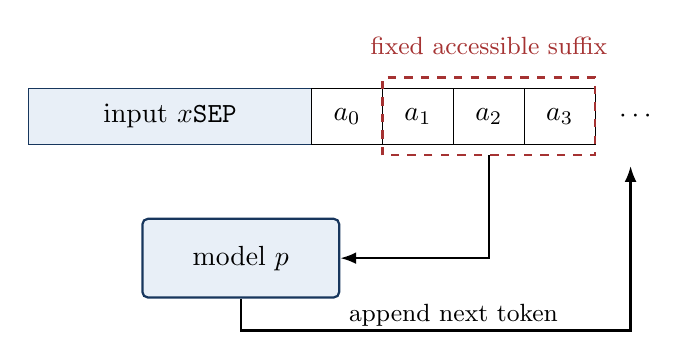
\begin{tikzpicture}[x=9mm,y=9mm]
\draw[fill=lightblue,draw=courseblue] (0,0) rectangle (4,0.8);
\node at (2,0.4) {input $x\sep$};
\foreach \j/\lab in {4/$a_0$,5/$a_1$,6/$a_2$,7/$a_3$}{
\draw (\j,0) rectangle +(1,0.8);\node at (\j+0.5,0.4) {\lab};}
\node at (8.6,0.4) {$\cdots$};
\draw[signalred,thick,dashed] (5,-0.15) rectangle (8,0.95);
\node[info,text=signalred] at (6.5,1.4) {fixed accessible suffix};
\node[module,minimum width=25mm] (p) at (3,-1.6) {model $p$};
\draw[flow] (6.5,-0.15) |- (p.east);
\draw[flow] (p.south) -- +(0,-0.45) -| (8.5,-0.3);
\node[info] at (6,-2.4) {append next token};
\end{tikzpicture}
\caption{An ever-growing transcript and a fixed accessible suffix provide
different memory interfaces. A transcript saved for display is not working
memory unless later computation can read it.}
\label{fig:window}
\end{figure}

\subsection{Bounded persistent state}

A \emph{configuration} records everything that can affect the subsequent
execution: controller state, accessible tokens, cache contents, and any
other persistent values. Time indices or position counters count if the
system can use them. We first consider a closed deterministic computation
after its input has been consumed, with no fresh external input.

\Needspace{8\baselineskip}
\begin{proposition}[A finite-state continuation]
\label{prop:finite-state}
Suppose the set $\cS$ of possible configurations has size at most $M$,
the transition is deterministic and independent of an external clock, and
the output stream supplies no readable state beyond the configuration.
Every execution either halts within $M$
transitions or eventually repeats a configuration and continues forever.
In the latter case, its sequence of emitted blocks is eventually periodic.
\end{proposition}
\begin{proof}
An execution taking more than $M$ transitions without halting visits some
configuration twice. Determinism makes the entire continuation from either
visit identical. A halt after the second visit would also have occurred
after the first, before completing the repeated segment. Therefore the
execution never halts, and its transitions and emitted blocks repeat.
\end{proof}

A fixed suffix of $K$ tokens has at most
$\sum_{j=0}^K|\Sigma|^j$ possible values. If the cache and other controller
state together use $B$ bits, the configuration count is bounded by
\begin{equation}
 M\leq 2^B\sum_{j=0}^K|\Sigma|^j.
 \label{eq:window-states}
\end{equation}
The bound can be enormous. Its significance is that a fixed amount of
persistent state cannot support every computation merely by running longer.
A bounded cache of contextualized activations generally carries more
information than the same number of raw token identities, but remains finite
at fixed precision.

Even exact real arithmetic inside a stateless map
$p:\Sigma^{\leq K}\to\Sigma$ leaves only finitely many
accessible suffixes. An exact real value retained between calls would change
the state model and could carry unbounded information. The distinction is
between arithmetic within a call and information retained across calls.

\begin{proposition}[Exact comparison requires retained information]
\label{prop:equality-stream}
A deterministic one-pass algorithm reads $u\#v$, where
$u,v\in\{0,1\}^{\ell}$, and must decide whether $u=v$. If no part of the
prefix can be reread, the state immediately after $u\#$ must have at least
$2^\ell$ possible values. A fixed-length binary encoding of that state
requires at least $\ell$ bits.
\end{proposition}
\begin{proof}
If fewer than $2^\ell$ states are available, two different prefixes
$u\#$ and $u'\#$ reach the same state. Supplying the common remaining input
$u$ then gives the same answer on $u\#u$ and $u'\#u$, although one answer
must be yes and the other no.
\end{proof}

The algorithm in this proposition includes the model and runtime together.
Every memory component that can affect the answer contributes to the state
count. Extra computation after a collision cannot recover the missing
distinction. A scratchpad from which the prefix can be recovered changes
the premises, and can remove this obstruction.

\subsection{An accessible growing context is a different case}

When the entire transcript remains accessible, the number of stored tokens
grows. Fixed precision per token does not bound total stored state. A
limitation then requires an argument about the actual attention and
positional mechanisms, rather than \eqref{eq:window-states} alone.

There are architecture-specific results in both directions. Under
causal attention, fixed-precision arithmetic, no positional embeddings, and a prescribed
left-to-right attention accumulation, one can summarize all future query
responses by finite state.\endnote{Finite attention state. Under the stated
numerical semantics, the possible queries form a finite set $\cQ$ and the
possible numerator--denominator accumulator values form a finite set
$\cB$. Retaining one accumulator for every query gives a head state in
$\cB^{\cQ}$, with at most $|\cB|^{|\cQ|}$ possibilities. Fixed numbers of
heads and layers preserve finiteness. The construction depends on the
absence of positional inputs and the specified accumulation rule.}
Conversely, specified hard-attention and relative
position mechanisms support universal simulation with a growing window.
The quantitative positive results are stated in \cref{sec:optional}.
Neither statement supplies a classification of every fixed-precision
transformer with growing context. The numerical operations and addressing
rules are part of the computational model.

\section{External memory and universal execution}
\label{sec:tape}

External memory can let a fixed model execute computations whose total state
is much larger than a single call. We now keep the model's architecture,
precision, and individual context budget fixed, and change the runtime.
Recall the finite transition rule of a
Turing machine. Let $Q$ be its finite control-state set, $\Gamma$ its finite
tape alphabet, and $Q_h\subseteq Q$ its halting states. A nonhalting
transition has the form
\begin{equation}
 \delta:(Q\setminus Q_h)\times\Gamma
 \longrightarrow Q\times\Gamma\times\{L,R\}.
 \label{eq:tm-rule}
\end{equation}
The runtime stores a tape, a head position, and the current control state.
If the control state belongs to $Q_h$, the runtime stops and returns the
tape's output under a fixed decoding convention. Otherwise it sends
$(q,a)$ to a model implementing $\delta$, receives
$(q',a',d)$, writes $a'$ in the current cell, moves one cell in direction
$d$, and retains $q'$. These are finite operations on one symbol at a time.
All queries come from the finite set $(Q\setminus Q_h)\times\Gamma$.
After finite input and output encodings, this is a small table. The
finite-context construction in \cref{thm:finite-table} shows that a finite
transformer can implement such a table with finite precision. The model
can emit the encoded transition tuple in a bounded number of token steps.

\begin{figure}[htbp]
\centering
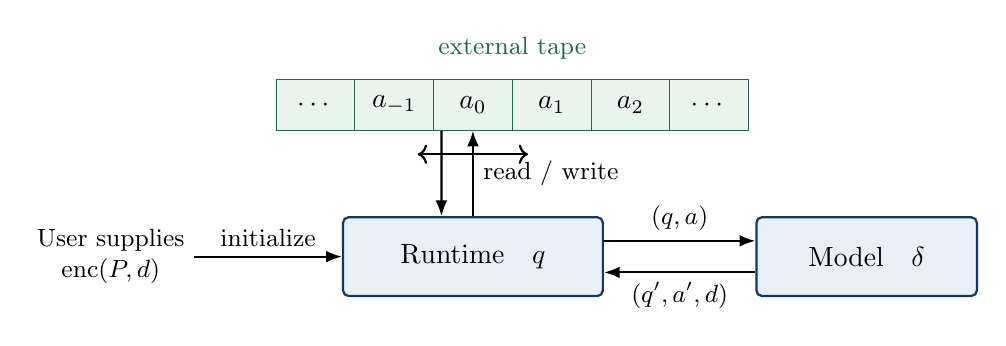
\begin{tikzpicture}[x=10mm,y=10mm]
\foreach \j/\lab in {0/$\cdots$,1/$a_{-1}$,2/$a_0$,3/$a_1$,4/$a_2$,5/$\cdots$}{
\draw[fill=lightgreen,draw=memorygreen] (\j,1.6) rectangle +(1,0.65);
\node at (\j+0.5,1.925) {\lab};}
\node[info,text=memorygreen] at (3,2.65) {external tape};
\node[module,minimum width=33mm] (rt) at (2.5,0) {Runtime\quad $q$};
\node[module,minimum width=28mm] (f) at (7.5,0) {Model\quad $\delta$};
\node[info] (usercode) at (-2.1,0) {User supplies\\$\enc(P,d)$};
\draw[flow] (usercode.east)--node[above,info]{initialize}(rt.west);
\draw[flow] (rt.north)--node[right,info]{read / write}(2.5,1.6);
\draw[flow] (2.1,1.6)--([xshift=-4mm]rt.north);
\draw[flow] ([yshift=2mm]rt.east)--node[above,info]{$(q,a)$}([yshift=2mm]f.west);
\draw[flow] ([yshift=-2mm]f.west)--node[below,info]{$(q',a',d)$}([yshift=-2mm]rt.east);
\draw[<->,thick] (1.8,1.3)--(3.2,1.3);
\end{tikzpicture}
\caption{Universal execution with a finite local model. The runtime
maintains the tape and location information; the model sees a state and
one tape symbol. The user must supply a program in the interpreter's
encoding.}
\label{fig:tape}
\end{figure}

If the local rule is that of a universal Turing machine, the combined system
can execute every computable program supplied in the appropriate input
encoding. The induction is the same as in Lecture 14: after each runtime
step, the external tape, head, and control state agree with the simulated
machine. A computation using $S$ tape cells does not require any individual
call to contain those $S$ cells. The runtime supplies the currently needed
symbol.

A fixed interpreter can execute many different programs because the program
to be executed is part of its input. In the universal-machine construction,
both $f$ and $R$ remain fixed. Let $P$ be a program in the machine's instruction
language, let $d$ be its input data, and let $\operatorname{enc}(P,d)$ encode
the pair on the initial tape. With a fixed output convention, the simulation
gives
\begin{equation}
 R^f\bigl(\operatorname{enc}(P,d)\bigr)=P(d).
 \label{eq:fixed-interpreter}
\end{equation}
The two sides have the same termination behavior: the runtime returns the
program's output if the program halts, and otherwise continues executing.
Changing $P$ changes the system input, without changing either $f$ or $R$.

The complete interpreter in \eqref{eq:fixed-interpreter} is $R^f$.
The model $f$ implements the universal machine's local transition rule;
the runtime $R$ stores and updates the tape, head position, and control
state. The analogy with a conventional interpreter concerns the division
between local computational rules and operations on execution state. The boundary
between $f$ and $R$ is a choice in our mathematical model; a Python
implementation need not have a separate component corresponding to $f$.

The construction places substantial work on the user: the desired task
must already have been translated into a program and encoded for the
interpreter. That is a familiar way to use a conventional computer, but
it leaves much of the intended AI capability unspecified. The model's
contribution in this construction is only a fixed local transition table.

For an AI system, the input $x$ should be allowed to contain instructions
in natural language together with data. Those instructions are code in
the language the system is expected to interpret. The design goal is a
generic runtime supplying memory and execution, while the model performs
substantial interpretation, decomposition, and synthesis. The user should
not have to compile each task into low-level transitions. We now hold a
\emph{given} model's reliable local capabilities fixed and ask how a
runtime can use them for long execution, extensive memory, or long output.

\section{The extension problem}
\label{sec:extension}

Prompting a model specifies a computational task: from the supplied
instruction and data, produce a suitable response. We idealize that task
by choosing one target answer for each valid request.\endnote{Tasks with
several acceptable answers. More generally, correctness is a relation
$V(x,y)$ on well-formed requests and responses. Invalid requests may be
excluded from the domain. Fixing a target $F(x)$ with $V(x,F(x))$ selects
one answer and makes the extension question deterministic. The lecture
assumes correctness on a trusted set; it does not assume that the runtime
has a verifier for arbitrary outputs. Verification-guided search is the
subject of Lecture 17.}
Let the target computation be
$F:D\to\Sigma^*$, where $D\subseteq\Sigma^*$, and let $W\subseteq D$
be a finite \emph{trusted set} whose membership is known or certified by
the construction. Assume
\begin{equation}
 f(w)=F(w)\qquad\text{for every }w\in W.
 \label{eq:trusted}
\end{equation}
No correctness assumption is made outside $W$. A possible competence
assumption is correctness whenever both the input and the required output
are short:
\begin{equation}
 \{w\in D:|w|\leq n,\ |F(w)|\leq m\}\subseteq W.
 \label{eq:length-trusted}
\end{equation}
The constants $n,m$ are call-length budgets in this lecture. The
description \eqref{eq:length-trusted} alone need not give an effective test
for membership in $W$, because $|F(w)|$ may be unknown. A runtime needs
either a known trusted request set or an argument that its requests belong
to that set.

\begin{definition}[Safe extension on an input]
\label{def:extension}
A runtime safely extends $F|_W$ to $x\in D$ if, using the oracle
$g=F|_W$, it makes only queries in $W$, halts, and returns $F(x)$.
Define its \emph{extension set} by
\begin{equation}
 E_R(F,W)=\{x\in D:R^{F|_W}(x)\text{ halts with }F(x)
                   \text{ using only queries in }W\}.
 \label{eq:extension-set}
\end{equation}
\end{definition}

For $x\in E_R(F,W)$, every model satisfying \eqref{eq:trusted} has the same
successful execution under $R$: the runtime never inspects untrusted
behavior. The central questions are whether $E_R(F,W)$ contains large
instances, how its size and structure depend on the runtime, and how many
calls and how much memory the extension uses.
The runtime $R_0$ that makes one unchanged model call has
\begin{equation}
 E_{R_0}(F,W)=W.
 \label{eq:trivial-extension}
\end{equation}
An extension result must explain which additional inputs a richer runtime
can solve using only that same trusted behavior.

The target structure must enter the problem somewhere. Two elementary
observations specify what an extension result has to assume.

\Needspace{7\baselineskip}
\begin{proposition}[Agreement on the trusted set does not determine an extension]
\label{prop:no-free-extension}
Suppose $x\in D\setminus W$ and two targets $F_1,F_2$ satisfy
$F_1|_W=F_2|_W$ but $F_1(x)\ne F_2(x)$. A fixed deterministic runtime,
given no information distinguishing the targets and querying only $W$,
cannot safely extend both targets to $x$.
\end{proposition}
\begin{proof}
The input and all oracle responses are identical in the two executions.
The executions therefore return the same answer if they halt.
\end{proof}

Conversely, allowing a separate unrestricted runtime $R_F$ for each
computable target makes extension immediate: $R_F$ can contain a complete
algorithm for $F$ and ignore the model. A useful result instead specifies a
generic execution mechanism, a structured task family, and the local
competence needed to operate that mechanism. A supplied decomposition or
program is legitimate input, but its computational contribution must be
identified.

For a stated task family $\cC$, runtimes can be compared by
\begin{equation}
 R_1\preceq_{\cC,W}R_2
 \quad\Longleftrightarrow\quad
 E_{R_1}(F,W)\subseteq E_{R_2}(F,W)\quad\text{for every }F\in\cC,
 \label{eq:runtime-order}
\end{equation}
where every $F$ has a domain containing $W$. The definition compares
particular runtimes: $R_2$ is at least as strong if every safe extension
achieved by $R_1$ is also achieved by $R_2$. Two runtimes can be incomparable,
and inclusion alone says nothing about their relative time or memory costs.
The task family, input representation, and trusted set are held fixed;
otherwise extra task-specific information could explain the difference.
Comparing memory architectures permits different
finite controllers within each architecture; the distinction will matter
in \cref{sec:stack}.
\endnote{Universal execution and extension. A universal oracle interpreter
can satisfy $U^g(\enc(R),x)=R^g(x)$ when it receives a program for $R$.
The interpreter does not determine which target is intended when several
targets agree on the available oracle answers.}

\section{Analysis, synthesis, and recursive execution}
\label{sec:recursion}

Recursive decomposition offers a way to use reliable short computations
repeatedly. The task structure will be a law expressing a problem's answer
through answers to subproblems. Retain the target
$F:D\to\Sigma^*$, let $D_{\mathrm{dec}}\subseteq D$ contain the inputs
on which decomposition is attempted, and let $\cJ\subseteq\Sigma^*$ be
the set of synthesis instructions. The \emph{analysis} and
\emph{synthesis} maps have types
\[
 A:D_{\mathrm{dec}}\to D\times D\times\cJ,
 \qquad S:\cJ\times\Sigma^*\times\Sigma^*\to\Sigma^*.
\]
Analysis replaces a problem $x$ by subproblems and a synthesis instruction:
\begin{equation}
 A(x)=(x_1,x_2,a).
 \label{eq:analysis}
\end{equation}
Synthesis maps the instruction $a$ and subproblem answers to an answer
for $x$. The required semantic identity is
\begin{equation}
 F(x)=S(a,F(x_1),F(x_2)).
 \label{eq:synthesis-law}
\end{equation}
Binary branching keeps the notation simple; any fixed maximum number of
children gives the same discussion.

The identity need not hold on every decomposable input. Define the
\emph{compatibility set}
\[
 \cC_F(A,S)=\{x\in D_{\mathrm{dec}}:
       F(x)=S(a,F(x_1),F(x_2))\}.
\]
Here $(x_1,x_2,a)=A(x)$ as in \eqref{eq:analysis}.
We call $(A,S)$ a \emph{sound decomposition of $F$ on $E$} when
$E\subseteq\cC_F(A,S)$. Recursive correctness follows when the identity
holds at every internal node reached, the direct leaf answers are correct,
and the recursion terminates. Membership of the root alone does not
establish those recursive premises.

When the analysis is realizable through the available interface, the
runtime obtains a decomposition of $x$, saves the
synthesis instruction $a$, solves the child problems recursively, and
then applies $S$. Synthesis may be performed by a model call, an algorithm
in the runtime, or a tool. A trusted direct call terminates the recursion
at a leaf. The saved instruction
belongs to the suspended parent call, so nested execution naturally uses
a stack.

Recursive language models use this ability to delegate work to further
model calls. Their execution environments may also store data and run
programs; those memory operations must be counted separately from the call
stack. Alternative-method search also fits the recursive structure.
Analysis can produce ``solve $x$ using method 1'' and ``solve $x$ using
method 2,'' with synthesis selecting a successful child result. Tree of
Thoughts uses branching over candidate reasoning steps, evaluation, and
search. Such branches can be treated as subproblems with a selection rule
for synthesis, with method-constrained requests or search states included
in $D$. For the fixed target $F$, selection must return the specified
answer $F(x)$. When several answers are acceptable, correctness is instead
expressed by the task's relation $V(x,y)$ from \cref{sec:extension}.
Selecting any successful child then requires correct success judgments
and branches that include a successful continuation whenever the parent
problem requires one. The recursive organization alone does not supply
these correctness guarantees.

\begin{figure}[htbp]
\centering
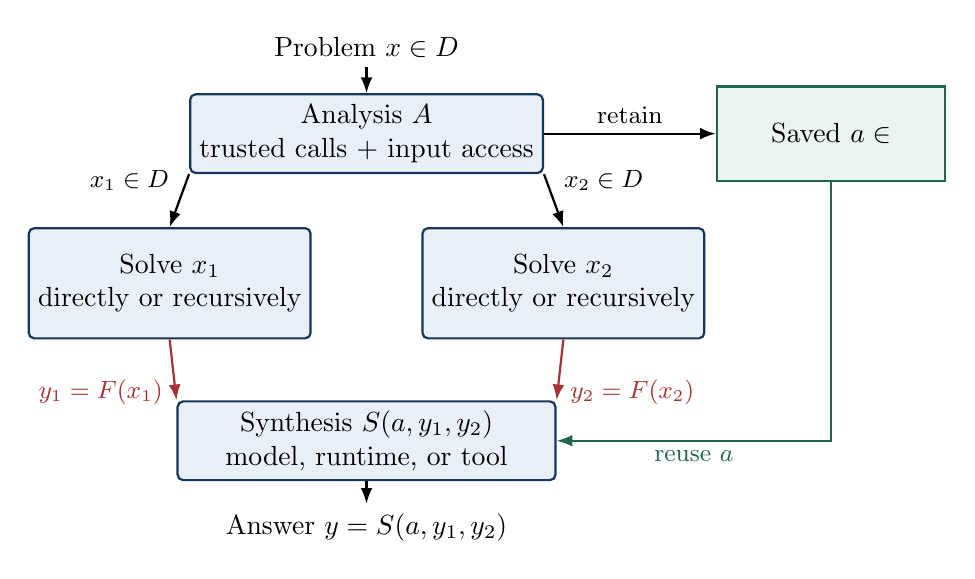
\begin{tikzpicture}[x=10mm,y=10mm]
\node (x) at (0,0) {Problem $x\in D$};
\node[module,minimum width=43mm] (analysis) at (0,-1.1)
 {Analysis $A$\\trusted calls + input access};
\node[module,minimum width=34mm,minimum height=14mm] (left) at (-2.5,-3)
 {Solve $x_1$\\directly or recursively};
\node[module,minimum width=34mm,minimum height=14mm] (right) at (2.5,-3)
 {Solve $x_2$\\directly or recursively};
\node[memory,minimum width=29mm,minimum height=12mm] (saved) at (5.9,-1.1)
 {Saved $a\in\cJ$};
\node[module,minimum width=48mm] (synth) at (0,-5)
 {Synthesis $S(a,y_1,y_2)$\\model, runtime, or tool};
\node (y) at (0,-6.1) {Answer $y=S(a,y_1,y_2)$};
\draw[flow] (x)--(analysis);
\draw[flow] (analysis.south west)--node[above left,info]{$x_1\in D$}(left.north);
\draw[flow] (analysis.south east)--node[above right,info]{$x_2\in D$}(right.north);
\draw[flow] (analysis.east)--node[above,info]{retain}(saved.west);
\draw[flow,signalred] (left.south)--node[below left,info]{$y_1=F(x_1)$}(synth.north west);
\draw[flow,signalred] (right.south)--node[below right,info]{$y_2=F(x_2)$}(synth.north east);
\draw[flow,memorygreen] (saved.south) |- node[below,pos=0.75,info]{reuse $a$}(synth.east);
\draw[flow] (synth)--(y);
\end{tikzpicture}
\caption{One recursive call, with analysis and synthesis separated.
Analysis produces subproblems $x_1,x_2$ and an instruction $a$. Each child
box may expand into another copy of this computation, ending in trusted
direct calls. The runtime retains $a$ while solving the children and then
supplies $a,y_1,y_2$ for synthesis. The arrows describe dependencies; a
stack runtime can execute the child calls sequentially. For a large $x$,
the analysis box denotes a protocol of bounded calls and runtime access,
whose realizability must be established.}
\label{fig:analysis-tree}
\end{figure}

\subsection{Which calls are assumed reliable?}

Correct direct answers do not automatically provide correct decompositions
or combinations. Let $\cQ\subseteq\Sigma^*$ be a set of encoded, tagged
requests, and let $F_{\mathrm{loc}}:\cQ\to\Sigma^*$ specify their answers.
If the model performs all three jobs, the specification includes three
request types. Suppressing the fixed tuple encodings, write
\begin{equation}
 \begin{aligned}
 F_{\mathrm{loc}}(\mathtt{solve},x)&=F(x),\\
 F_{\mathrm{loc}}(\mathtt{analyze},d)&=\text{an encoded decomposition from the local view }d,\\
 F_{\mathrm{loc}}(\mathtt{synthesize},a,y_1,y_2)&=S(a,y_1,y_2).
 \end{aligned}
 \label{eq:three-requests}
\end{equation}
Let $W_{\mathrm{loc}}$ be the finite trusted set of these encoded requests.
The new competence assumption is $f(q)=F_{\mathrm{loc}}(q)$ for $q\in W_{\mathrm{loc}}$.
The local competence assumption is stronger than knowing only
\eqref{eq:trusted} for direct questions.
An equivalent formulation uses one target function on a domain containing
all the tagged request types.

A \emph{synthesis request} is the encoded input
\[
 q_{\mathrm{syn}}=\enc(\mathtt{synthesize},a,y_1,y_2)\in\Sigma^*.
\]
When the model implements $S$, the entire request must belong to
$W_{\mathrm{loc}}$. An input-length budget therefore applies jointly to
the instruction, both child answers, and their encoding. Short child
answers alone do not establish that the synthesis call is trusted.
When a tool implements $S$, its input limits, memory, and correctness
assumptions replace the model's synthesis-call requirement. The following
supplied-tree analysis studies the case where the model implements $S$.

In particular, writing $A(x)=f(\mathtt{analyze},x)$ does not justify sending
an arbitrarily long $x$ to a model trusted only on short contexts. The
runtime must already be able to present a bounded description of the next
decomposition operation, or the input must supply the organization. A
short name for a large object is useful only when the runtime also defines
how that object can be accessed. The stored object remains part of the
system's memory.

We start with a supplied decomposition tree. Every leaf contains a bounded
direct problem, and every internal node contains a bounded synthesis
instruction. A parenthesized serialization lets a parser read the tree in
depth-first order using a stack. No model call needs to contain the whole
tree. The model is responsible for solving the leaf problems and performing
the prescribed synthesis operations.

\subsection{The runtime's stack}

A \emph{stack} stores frames with last-in, first-out access. The runtime can
inspect and modify the top frame, push a new frame, or pop the top frame.
A suspended recursive call needs a synthesis instruction, a record of which
child is being processed, and any completed child answer. These values form
its \emph{call frame}.

\Needspace{11\baselineskip}
For a supplied binary tree, the abstract execution is:
\begin{lstlisting}
Evaluate(node):
    if node is a leaf:
        return Model(solve, node.description)
    save node.instruction in a call frame
    y1 = Evaluate(first child)
    save y1 in the frame
    y2 = Evaluate(second child)
    return Model(synthesize, node.instruction, y1, y2)
\end{lstlisting}
Here ``node'' is explanatory notation. In the one-way implementation the
parser consumes delimiters, leaf descriptions, and instructions from the
serialized input; it does not retain arbitrary node pointers. Siblings are
read when their turn arrives. The stack retains only bounded local data.

\begin{figure}[htbp]
\centering
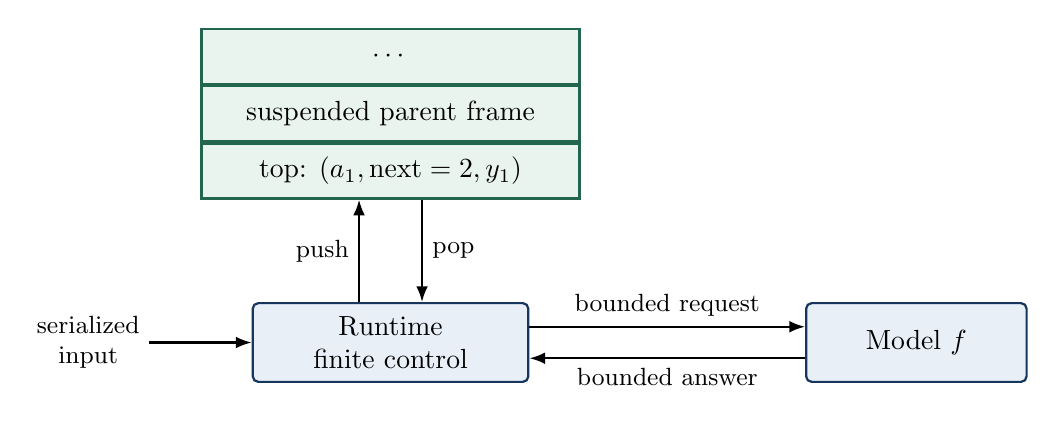
\begin{tikzpicture}[node distance=20mm]
\node[module,minimum width=35mm] (rt) {Runtime\\finite control};
\node[module,minimum width=28mm,right=35mm of rt] (f) {Model $f$};
\node[memory,minimum width=48mm,minimum height=7mm,above=13mm of rt] (top) {top: $(a_1,\text{next}=2,y_1)$};
\node[memory,minimum width=48mm,minimum height=7mm,above=0mm of top] (old) {suspended parent frame};
\node[memory,minimum width=48mm,minimum height=7mm,above=0mm of old] (bottom) {$\cdots$};
\draw[flow] ([xshift=-4mm]rt.north)--node[left,info]{push}([xshift=-4mm]top.south);
\draw[flow] ([xshift=4mm]top.south)--node[right,info]{pop}([xshift=4mm]rt.north);
\draw[flow] ([yshift=2mm]rt.east)--node[above,info]{bounded request}([yshift=2mm]f.west);
\draw[flow] ([yshift=-2mm]f.west)--node[below,info]{bounded answer}([yshift=-2mm]rt.east);
\node[info,left=13mm of rt] (input) {serialized\\input};
\draw[flow] (input)--(rt);
\end{tikzpicture}
\caption{The stack stores suspended calls outside the active model context.
Each frame can be bounded even when the stack depth grows. The bottommost
drawn frame is the accessible top of the stack.}
\label{fig:stack}
\end{figure}

\Needspace{12\baselineskip}
\begin{proposition}[Correct composition with a supplied decomposition]
\label{prop:composition}
Let a finite binary decomposition tree have $N$ nodes and height $h$,
counting nodes on a longest root-to-leaf path. Assume every leaf call and
every synthesis call arising on correct child answers belongs to
$W_{\mathrm{loc}}$. Assume the synthesis identity
\eqref{eq:synthesis-law} at every internal node. Then the recursive runtime
returns $F(x)$ using $N$ model calls. If instructions and answers use at most
$b$ bits each, the one-way implementation uses $O(hb+h)$ stack bits, besides
the bounded workspace of one model call.
\end{proposition}
\begin{proof}
At a leaf, correctness follows from the local competence assumption.
Inductively, both children return their specified answers. The synthesis
request is therefore trusted and returns the parent's answer by
\eqref{eq:synthesis-law}. Every node invokes the model once. At most $h$
frames are active, each holding a bounded instruction, one child answer,
and a finite execution phase.
\end{proof}

The proposition specifies what has to be checked for a decomposition to
extend local competence. A large tree can satisfy these premises without
any large individual call. The substantive difficulty is finding suitable
subproblems and sufficiently informative bounded answers. Recursion alone
does not establish the synthesis identity or the trusted-call premise.
For a model-generated tree, one must additionally establish correct
analysis calls and termination, for example by a nonnegative integer rank
that strictly decreases on every child.

\section{The limitation of one stack}
\label{sec:stack}

The supplied-tree evaluator can process arbitrarily many nested subproblems
while each model call and each saved answer remain bounded. Does an
unbounded call stack suffice for general problem solving? The answer depends
on what a call frame contains and how the system can read its input.

We first study yes/no tasks. A \emph{decision problem} on strings is
identified with its \emph{language} $L\subseteq\Sigma^*$, the set of inputs
whose correct answer is yes. A system \emph{accepts} an input when it
terminates with answer yes. It \emph{decides} $L$ when it terminates
on every input and returns yes exactly on the members of $L$. A universal
instruction-following system must handle these tasks among its other tasks,
so a limitation for decision problems already limits that ambition.
\endnote{String outputs and decisions. For a total string-valued computation,
questions about whether the output has a given length or symbol are
decision problems. Such encodings do not remove output cost: writing $m$ symbols
still takes at least $m$ output operations. We use decision problems for the
separations and retain the separate output resource for constructive results.}

\begin{definition}[Finite control with one stack]
\label{def:pushdown}
A \emph{pushdown system with one-way input} has a finite controller, a stack
over a finite alphabet $\Gamma$, and a read-only input head that can advance
but cannot move backward. A transition depends on the controller state,
the top stack symbol, and the next input symbol or an end marker. A
transition may leave the input head in place. It changes the controller
state and replaces the top stack symbol by a string of bounded length.
The transition rule specifies a unique next step whenever execution
continues. An output stream, if present, is write-only.
\end{definition}

\emph{Finite persistent control} means that all information retained outside
the declared input and stack takes values in one fixed finite set,
independent of input length. The control includes local notes, pending-call
information, bounded call buffers, and any bounded finite-precision cache.
Finitely many possible bounded call frames can serve as the stack alphabet.
Input locations saved as arbitrarily large integers are excluded here.

\begin{theorem}[The limitation of a single stack]
\label{thm:stack}
A runtime with finite persistent control, one-way input, one stack of
bounded frames, and a model called only on a fixed finite trusted set can
be simulated by a pushdown automaton. Its accepted input language is
context-free. In particular, it cannot decide
\begin{equation}
 L_3=\{a^j b^j c^j:j\geq1\}.
 \label{eq:three-blocks}
\end{equation}
\end{theorem}
\begin{proof}
Include the bounded runtime data and model-call phase in the finite
controller. The possible frames form a finite stack alphabet. Every
trusted model request has a fixed terminating response, so its effect can
be included in the finite transition rule. The resulting system has exactly
the operations of \cref{def:pushdown}.

The languages accepted by pushdown automata are context-free: they admit
grammars whose production rules replace one nonterminal at a time. The
language $L_3$ is not context-free, as proved in
\appendixref{app:pumping}. Hence no system satisfying the premises decides
$L_3$.
\end{proof}

\subsection{What the theorem says about following an instruction}

The theorem rules out a concrete instruction-following guarantee. Let
$I_3\in\Sigma^*$ be the fixed token string encoding this prompt, including
the delimiter immediately before the supplied data:
\begin{quote}
Answer Yes exactly when the following string consists of a positive number
of a's, followed by the same number of b's, followed by the same number of
c's. Otherwise answer No. The string is:
\end{quote}
Append $w\in\{a,b,c\}^*$ to obtain the complete request $I_3w$. The
specified answer is the map
\begin{equation}
 d_3:\{a,b,c\}^*\to\{\mathtt{Yes},\mathtt{No}\},\qquad
 d_3(w)=\begin{cases}\mathtt{Yes},&w\in L_3,\\
                         \mathtt{No},&w\notin L_3.
          \end{cases}
 \label{eq:three-block-instruction}
\end{equation}
For example, $d_3(\mathtt{aabbcc})=\mathtt{Yes}$ and
$d_3(\mathtt{aabbbcc})=\mathtt{No}$. Reliable execution of the instruction
would mean $R^f(I_3w)=d_3(w)$ for every appended string $w$.

\begin{corollary}[A fixed instruction that the one-stack system cannot always execute]
\label{cor:stack-instruction}
Let $R$ and $f$ satisfy the premises of \cref{thm:stack}. Suppose the system
returns either $\mathtt{Yes}$ or $\mathtt{No}$ on every request $I_3w$.
Then
\begin{equation}
 \exists w\in\{a,b,c\}^*:\quad R^f(I_3w)\ne d_3(w).
 \label{eq:stack-instruction-failure}
\end{equation}
If the system returns only Yes or No but is allowed not to terminate,
then it must answer incorrectly or fail to terminate on some such request.
\end{corollary}
\begin{proof}
Suppose every request receives the correct answer. Construct a machine on
input $w$ that simulates $R^f$ with the fixed prefix $I_3$ supplied first,
then supplies the symbols of $w$. The index into $I_3$ has finitely many
possible values because $I_3$ is fixed. The simulation preserves every
stack operation and needs only finite additional control. It is therefore
a one-stack machine deciding $L_3$, contrary to \cref{thm:stack}.
\end{proof}

The instruction has fixed length, and the requested answer is one of two
fixed strings. Only the data grows. Even a model that understands the
instruction perfectly cannot execute it on every input through this
restricted runtime. Understanding the instruction and providing the memory
access needed to carry it out are separate requirements.

The proof simulates the system's actual processing of $I_3$; it does not
supply an interpreter for natural language. Likewise, including bounded
model behavior in a finite transition rule is an upper-bound argument,
not a proposed implementation of language understanding.

The supplied-tree evaluator satisfies the theorem's premises when its input
is consumed once and its local labels and answers have fixed bounds.
Conventional recursive software often saves references to the original
input, however. A saved reference lets a later call revisit a passage that
the input head has already passed. We next add this operation and examine
how much computational power it provides.

\section{Recursive calls with references to the input}
\label{sec:readonly}

The next runtime retains the original request and lets recursive calls
save locations in it. A model can ask to revisit a passage after a child
call has finished. We call this a \emph{read-only recursive runtime}:
the input remains unchanged, and saved references initially point only
into that input. The question is how far this added access extends what
the system can do.

\subsection{What the runtime stores and what the model requests}

Each call frame has a fixed number of named slots, such as $u,v,z$, for
input references, together with bounded notes. A reference to position $i$
denotes the suffix $x_i\cdots x_n$ of the retained request $x$. The runtime
handles the address; the model names a slot. In formulas, $u$ denotes the
referenced suffix string; the runtime stores its starting position.
For a fixed positive view length $c$, define
\[
 \operatorname{view}_c:\Sigma^*\to\Sigma^{\leq c},\qquad
 \operatorname{view}_c(u)=\operatorname{prefix}_c(u).
\]
A local request can contain a control label $\ell$, a bounded note $b$,
and short passages obtained from saved locations:
\begin{equation}
 q=\enc\bigl(\ell,b,\operatorname{view}_c(u),
                    \operatorname{view}_c(v)\bigr)\in W_{\mathrm{loc}}.
 \label{eq:reference-request}
\end{equation}
The model can classify these passages, decide how to proceed, or combine
bounded answers. Its reply selects from a fixed finite vocabulary of
operations on the named slots. A representative interface is:
\begin{center}
\small
\renewcommand{\arraystretch}{1.15}
\begin{tabular}{p{0.32\textwidth}p{0.60\textwidth}}
\toprule
Operation & Runtime action \\
\midrule
$\mathtt{inspect}(u)$ & Supply $\operatorname{view}_c(u)$ to a local call \\
$v\leftarrow u$ & Save the same input location in another slot \\
$u\leftarrow\mathtt{tail}(u)$ & Advance that reference by one token \\
$\mathtt{call}\ j(v,b)$ & Save the parent frame and start the named child procedure \\
$\mathtt{return}(u)$ & Restore the parent frame and return the value in the named slot \\
\bottomrule
\end{tabular}
\end{center}
Slot names and procedure names range over fixed finite sets. Copying a
reference does not copy its suffix. For example, a call can save $u$,
recurse from $v$, then inspect $u$ again when the child returns. The child
has its own reference slots, so advancing a child slot preserves the saved
parent location. All calls to the model must satisfy the trusted-set
condition in \eqref{eq:reference-request}.

This interface keeps the model's observations bounded while permitting
repeated access to a large request. We now specify the permissible values
and control precisely; those restrictions will determine the theorem.

\subsection{A precise read-only interface}

Fix an input $x=x_1\cdots x_n$. Let $B$ be a fixed finite set of bounded
values, containing token observations, Boolean answers, control labels,
and any bounded model responses. Write
\begin{equation}
 \operatorname{Suf}(x)=\{x_i\cdots x_n:1\leq i\leq n+1\},
 \qquad V_x=B\mathbin{\dot\cup}\operatorname{Suf}(x).
 \label{eq:readonly-values}
\end{equation}
The suffix with $i=n+1$ is empty. The disjoint union keeps a bounded token
value distinct from a reference to a one-token suffix. A suffix is stored
as its input position, using $O(\log(n+2))$ bits, rather than as a copy of
its contents.

\begin{definition}[Read-only recursive runtime and its call protocols]
\label{def:readonly}
A runtime in this class executes a fixed finite \emph{call protocol} $P$.
The protocol consists of finitely many named recursive procedures, each
with a fixed finite number of parameters and local variables taking values
in $V_x$. Procedure bodies use the following operations:
\begin{enumerate}[label=(\roman*),leftmargin=*]
\item inspect the first symbol of a nonempty suffix, test whether a suffix
is empty, and obtain its tail;
\item copy existing values, use constants in $B$ and the empty suffix,
and apply fixed functions $g:B^r\to B$ of fixed arity, including trusted
model calls on bounded requests;
\item branch on a Boolean value, bind a local variable, call a named
procedure with evaluated arguments, and return a value in $V_x$.
\end{enumerate}
Evaluation is sequential and call-by-value: arguments are evaluated before
entering a procedure. Calls have no side effects and cannot inspect the
caller's frame. There are no other data operations or stores. In particular,
functions are not values that can be passed or returned; this is the
\emph{first-order} restriction. The entry procedure receives $x$ as a suffix
reference and, for a decision problem, returns a Boolean value.
\end{definition}

Write $R_P^f$ for execution of protocol $P$ using model $f$. The protocol
specifies how calls and runtime operations are combined; model calls
remain responsible for their specified local computations. A bounded view
is implemented by at most $c$ reads and $c$ advances. Notes and
references that affect a procedure's result must be explicit arguments;
the procedure has no hidden persistent state. A command loop can be
written as tail-recursive calls carrying its control label and current
slots as arguments.

The interface implements analysis as recursive calls on selected input
references, direct solution through trusted local operations, and synthesis
through bounded returns or further recursive computations. The input can
include both instructions and data in one string. The definition grants
access to that string without granting an interpretation of its contents.

The mathematical name for these protocols is \emph{first-order cons-free
recursion}: functions cannot be passed as values, and the operation
\texttt{cons} for constructing a new list cell is absent. We will use a
theorem about this class to determine the power of the specified runtime.
\endnote{Scope of the read-only restriction. The value set and first-order
restriction are essential. An ordinary program may have read-only input
while allocating large intermediate strings, integers, or function closures.
Such values are not in $V_x$. Higher-order cons-free languages have different
complexity characterizations; passing functions as data is therefore not an
innocuous change to \cref{def:readonly}.}

\begin{figure}[htbp]
\centering
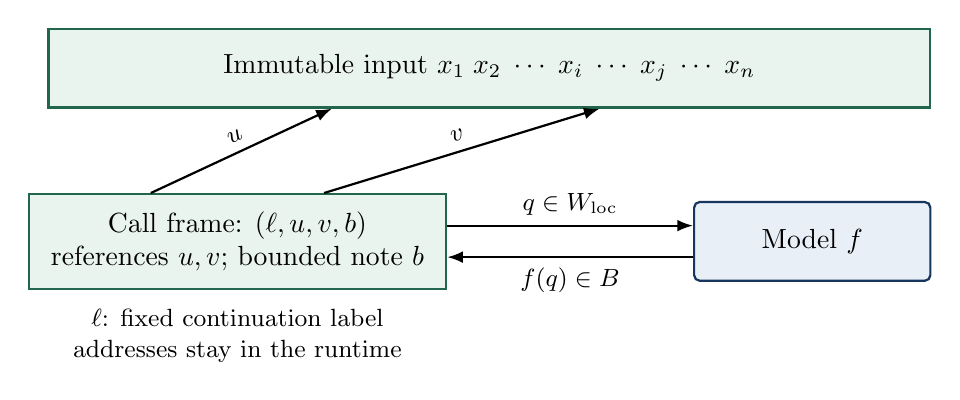
\begin{tikzpicture}[x=10mm,y=10mm]
\node[memory,minimum width=112mm,minimum height=10mm] (input) at (0,2.2)
 {Immutable input $x_1\;x_2\;\cdots\;x_i\;\cdots\;x_j\;\cdots\;x_n$};
\node[memory,minimum width=53mm,minimum height=12mm] (frame) at (-3.2,0)
 {Call frame: $(\ell,u,v,b)$\\references $u,v$; bounded note $b$};
\node[module,minimum width=30mm] (model) at (4.1,0) {Model $f$};
\node[info] at (-3.2,-1.2) {$\ell$: fixed continuation label\\addresses stay in the runtime};
\draw[flow] ([xshift=-11mm]frame.north)--node[above,sloped,info]{$u$}([xshift=-20mm]input.south);
\draw[flow] ([xshift=11mm]frame.north)--node[above,sloped,info]{$v$}([xshift=14mm]input.south);
\draw[flow] ([yshift=2mm]frame.east)--node[above,info]{$q\in W_{\mathrm{loc}}$}
 ([yshift=2mm]model.west);
\draw[flow] ([yshift=-2mm]model.west)--node[below,info]{$f(q)\in B$}
 ([yshift=-2mm]frame.east);
\end{tikzpicture}
\caption{A recursive frame can retain references without exposing their
numerical addresses to the model. Unlike a frame drawn from a fixed finite
alphabet, this frame needs $O(\log(n+2))$ bits on a length-$n$ input.
The runtime can revisit the referenced input after other calls return.}
\label{fig:input-references}
\end{figure}

\subsection{Executing the same instruction with saved references}

Return to the request $I_3w$ from \cref{cor:stack-instruction}. Once the
system selects the prescribed block test, saved input references suffice
to execute it. First scan the data string $w$ to
check that it has the form $a^+b^+c^+$, retaining references $u,v,z$ to the
starts of the three blocks. Then advance the three references together,
one symbol per step. Accept exactly when all three references reach the
ends of their respective blocks on the same step. Testing a block end
requires only the next token or the empty-suffix test. The scans use fixed
finite control and can be written as tail-recursive procedures.

On the data $\mathtt{aaabbbccc}$ the simultaneous scan is:
\begin{center}
\begin{tabular}{c c c c}
\toprule
Step & $u$ denotes & $v$ denotes & $z$ denotes \\
\midrule
0 & $\mathtt{aaabbbccc}$ & $\mathtt{bbbccc}$ & $\mathtt{ccc}$ \\
1 & $\mathtt{aabbbccc}$ & $\mathtt{bbccc}$ & $\mathtt{cc}$ \\
2 & $\mathtt{abbbccc}$ & $\mathtt{bccc}$ & $\mathtt{c}$ \\
3 & $\mathtt{bbbccc}$ & $\mathtt{ccc}$ & $\epsilon$ \\
\bottomrule
\end{tabular}
\end{center}
The runtime stores three locations, not three copied strings. A local call
needs only the three current symbols and the scan phase. All three block
ends are reached together in the last row, so the answer is
$\mathtt{Yes}$. If the block lengths differ, the block ends are reached
on different steps.

\begin{proposition}[Saved input references exceed the one-stack restriction]
\label{prop:three-references}
The interface of \cref{def:readonly} decides $L_3$ with $O(n)$ primitive
operations on an input of length $n$.
\end{proposition}
\begin{proof}
The initial scan checks the order and nonemptiness of the blocks. The
simultaneous scan accepts exactly when their three positive lengths agree.
Each scan advances its references at most $n$ times and performs a bounded
number of operations per step. Tail recursion implements the scans using
the permitted operations.
\end{proof}

The gain comes from saved access to several input positions. The number
of values a reference can take grows with $n$, so the frames no longer
satisfy the finite-alphabet premise of \cref{thm:stack}. The model's local
observation and answer lengths can remain fixed throughout both scans.
In the notation for the requested system behavior, a protocol $P_3$ that
correctly dispatches $I_3$ to this scan satisfies
\begin{equation}
 R_{P_3}^f(I_3w)=d_3(w)\qquad(w\in\{a,b,c\}^*),
 \label{eq:reference-instruction-success}
\end{equation}
provided its interpretation and scan calls are trusted and correct.
The memory obstruction has been removed; the model's required local
competence is still an assumption.

\section{The computational power of read-only recursion}
\label{sec:readonly-power}

Saved references let the runtime execute the three-block instruction that
one-way input and a stack could not support. We now ask how far this
extension goes when execution time is unrestricted. The answer is an exact
characterization of the decision tasks supported by the read-only interface.

A decision problem is in $\mathsf P$ if some algorithm decides every
length-$n$ input in at most $C(n+1)^d$ steps, for fixed constants $C,d$.
The constants may depend on the problem and algorithm, but not on the
particular input. We count finite-bit operations; references can be encoded
by integers with $O(\log(n+2))$ bits.

\begin{theorem}[Decision tasks supported by the read-only runtime]
\label{thm:cons-free}
A language $L\subseteq\Sigma^*$ is decided by some call protocol and
bounded local functions permitted by \cref{def:readonly}, using ordinary
recursive evaluation without a time bound, if and only if
$L\in\mathsf P$.
\end{theorem}

The theorem concerns which tasks the original runtime can solve, even if
its executions take much longer than polynomial time. For any fixed protocol
and bounded local functions that decide a language, there is a polynomial-time
algorithm giving the same answers. Conversely, every language in $\mathsf P$
has some permitted protocol and bounded local functions. Those choices may
depend on the language, but remain fixed as the input length grows.
A particular model's trusted repertoire may support fewer tasks; a positive
extension claim still requires correct execution using only trusted calls.

We prove the upper bound by constructing an equivalent evaluator that
remembers completed calls. The evaluator's cache is a device in the proof;
the runtime being characterized need not have that cache. The converse is
a classical expressivity theorem for cons-free programs, stated here without
proof.

\subsection{Auxiliary lemma: polynomially many distinct calls}

A recursive execution can revisit the same subproblem many times. We identify
a complete call by its procedure and arguments, then evaluate each distinct
call only once. The resulting evaluator is called \emph{memoized evaluation}.
Write $\widehat R_P^f$ for this evaluator applied to protocol $P$ and model $f$.
The required relation is
\begin{equation}
 \widehat R_P^f(x)=R_P^f(x)
 \qquad\text{whenever }R_P^f(x)\text{ terminates}.
 \label{eq:cache-preservation}
\end{equation}
The evaluator stores completed results in a cache. The protocol's operations
remain those of \cref{def:readonly}: it cannot inspect or modify cache
entries, observe cache hits, or query elapsed time. Purity ensures that
reusing a completed result preserves the computation.

Let $j$ name a procedure of arity $r_j$. A complete call has key
\begin{equation}
 \kappa=(j,v_1,\ldots,v_{r_j}),\qquad v_i\in V_x.
 \label{eq:call-key}
\end{equation}
The cache is reset for each original input $x$. Within that evaluation, a
suffix argument is identified by its position in $x$. All notes that affect
the result must be explicit arguments; local variables are computed from
them. A cache entry stores the returned value $v\in V_x$.

\begin{lstlisting}
Evaluate(j, arguments):
    key = (j, arguments)
    if key has a completed entry:
        return cache[key]
    mark key active
    value = evaluate body j on arguments
            using Evaluate for recursive calls
    cache[key] = value
    mark key completed
    return value
\end{lstlisting}
An attempt to reenter an active key certifies nontermination of that call
under these semantics. Repeating the same pure call repeats the same
unfinished dependencies. A runtime can report this cycle separately; it
must not substitute a fabricated answer. For a protocol that terminates on
every input, no active key is reentered.

\Needspace{11\baselineskip}
\begin{lemma}[Polynomial-time evaluation of a read-only protocol]
\label{lem:memoized}
Fix a program $P$ as in \cref{def:readonly}, with $q$ procedures and maximum
arity $k\geq1$. The memoized evaluator returns the same value as ordinary
evaluation on every length-$n$ input where ordinary evaluation terminates.
On such an input, it evaluates at most
\begin{equation}
 M_P(n)=q\bigl(n+1+|B|\bigr)^k
 \label{eq:call-count}
\end{equation}
procedure bodies. It uses $O(M_P(n)\log(n+2))$ auxiliary bits and admits
a polynomial-time implementation.
\end{lemma}
\begin{proof}
All arguments and results belong to $V_x$, which has $n+1+|B|$ elements.
For procedure $j$ there are at most $|V_x|^{r_j}$ possible argument tuples.
Summing over the $q$ procedures gives at most $M_P(n)$ keys.

Purity makes a call's result a function of its key. On a terminating
execution, a key cannot recur among its own active ancestors: the later
call would reproduce the same unfinished computation indefinitely. A key
is therefore evaluated once and then served from the completed cache.
Induction over completed calls shows that every cached value equals the
ordinary evaluation's result.

A procedure body has fixed size. Outside its recursive calls, evaluating
that body performs only a fixed number of primitive operations, local
bindings, and cache accesses. There are $O(M_P(n))$ such operations and
cache accesses in total. Keys, results, and frames each need
$O(\log(n+2))$ bits, and at most $M_P(n)$ keys can be active or completed.
The auxiliary-space bound follows. Storing the cache as a searchable list
already gives polynomial lookup cost; more efficient dictionaries can be
used. Input access and operations on encoded references also have polynomial
bit cost. Thus the total bit cost is polynomial in $n$.
\end{proof}

\begin{proof}[Proof of the upper bound in \cref{thm:cons-free}]
Suppose a protocol decides a language $L$ under ordinary evaluation.
It terminates on every input. By \cref{lem:memoized}, the memoized evaluator
returns the same answers in polynomial time. Thus
\[
 R_P^f\text{ decides }L
 \quad\Longrightarrow\quad
 \widehat R_P^f\text{ decides }L\text{ in polynomial time}
 \quad\Longrightarrow\quad L\in\mathsf P.
\]
\end{proof}

Allowing more time for the original protocol cannot make it decide a
language outside $\mathsf P$. The next example turns that restriction into
an instruction-following limitation.

\subsection{A limitation illustrated by generalized chess}

The polynomial bound rules out some computable tasks that naturally invite
recursive search. Consider the following decision task: given a chess
position on a variable-size board, can a designated player force a win?
The board size is part of the instance. The generalization retains the
usual piece movements, allows the number of pieces to grow with the board,
and treats indefinite play without a forced win as nonwinning. There is no
fixed or polynomial move limit imposed on the game. The result below uses
the standard generalized-chess family specified in the bibliographical
notes; it concerns arbitrary supplied positions, not only positions reached
from a particular opening.

The class $\mathsf{EXPTIME}$ consists of decision problems solvable within
$2^{n^{O(1)}}$ time. A problem is \emph{EXPTIME-complete} if it belongs to
this class and every problem in the class can be transformed into it by a
polynomial-time computation preserving yes/no answers.

\begin{theorem}[Generalized chess; stated without proof]
\label{thm:chess}
Determining whether a designated player can force a win in the specified
generalization of chess is EXPTIME-complete. Moreover,
$\mathsf P\subsetneq\mathsf{EXPTIME}$.
\end{theorem}

\begin{corollary}[The read-only recursive interface does not suffice for chess]
\label{cor:readonly-chess}
Let $I_{\mathrm{chess}}$ be a fixed instruction asking whether the designated
player can force a win in the generalized-chess position supplied after it.
Let $\cB\subseteq\Sigma^*$ be the valid position encodings, and let
$\operatorname{Win}:\cB\to\{\mathtt{Yes},\mathtt{No}\}$ specify the correct
answer. For any fixed protocol $P$ and model $f$ satisfying
\cref{def:readonly}, if $R_P^f(I_{\mathrm{chess}}w)$ returns Yes or No for
every $w\in\cB$, then
\begin{equation}
 \exists w\in\cB:\quad R_P^f(I_{\mathrm{chess}}w)\ne\operatorname{Win}(w).
 \label{eq:chess-instruction-failure}
\end{equation}
The statement also holds for $\widehat R_P^f$. Perfect local calls and
unrestricted execution time do not remove the limitation.
\end{corollary}
\begin{proof}
If all these answers were correct, \cref{lem:memoized} would give a
polynomial-time algorithm for generalized chess: check the position
encoding, prepend the fixed instruction, and evaluate the protocol with
caching. Validity of the full board encoding is checkable in polynomial
time; invalid encodings can be rejected. The fixed prefix changes input
length by a constant. Completeness would then put every EXPTIME problem
in $\mathsf P$, contradicting \cref{thm:chess}.
\end{proof}

The separation is unconditional; it does not depend on whether
$\mathsf P=\mathsf{NP}$. It concerns exact answers for unbounded board sizes,
so it makes no claim about the quality of play on a fixed $8\times8$ board.
The instruction-following conclusion has the same form as
\cref{cor:stack-instruction}, now for the stronger runtime. The system can
reread the entire supplied position and make arbitrarily many recursive
calls. Nevertheless, for some supplied position, it cannot return the
correct answer through this interface. The limitation concerns the
permitted persistent values, even when every local semantic decision is
correct.

\subsection{Implementation consequence: caching completed calls}
\label{sec:memoization}

The evaluator used in the proof can also be implemented as a runtime
improvement. It reuses the answer to a completed recursive call, including
all model calls and input inspections that would otherwise be repeated.
The model, local prompts, and permitted answers remain unchanged.

Read-only recursion permits very long executions. The following program
deliberately solves the same suffix problem twice. Both calls are evaluated
before their answers are combined.
\begin{lstlisting}
Repeat(u):
    if empty(u): return True
    a = Repeat(tail(u))
    b = Repeat(tail(u))
    return a and b
\end{lstlisting}
If $C(n)$ counts procedure-body evaluations on a length-$n$ input, then
\begin{equation}
 C(0)=1,\qquad C(n)=1+2C(n-1)=2^{n+1}-1.
 \label{eq:repeat-cost}
\end{equation}
Every call returns true. The execution takes exponentially many steps even
though the task has a constant answer. There are only $n+1$ distinct calls,
one per suffix, so memoization reduces the number of procedure-body
evaluations from $2^{n+1}-1$ to $n+1$.

\begin{figure}[htbp]
\centering
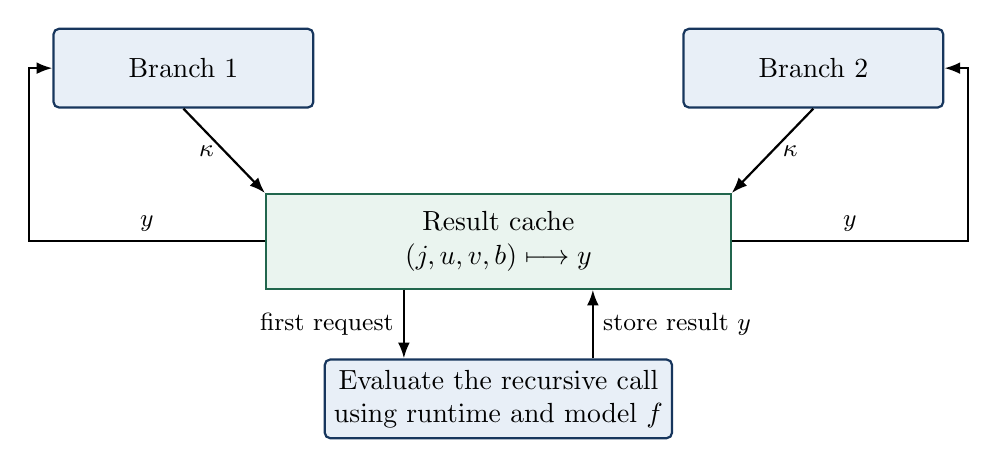
\begin{tikzpicture}[x=10mm,y=10mm]
\node[module,minimum width=33mm] (left) at (-4,2.2) {Branch 1};
\node[module,minimum width=33mm] (right) at (4,2.2) {Branch 2};
\node[memory,minimum width=59mm,minimum height=12mm] (cache) at (0,0)
 {Result cache\\$(j,u,v,b)\longmapsto y$};
\node[module,minimum width=43mm] (eval) at (0,-2)
 {Evaluate the recursive call\\using runtime and model $f$};
\draw[flow] (left.south)--node[left,info]{$\kappa$}(cache.north west);
\draw[flow] (right.south)--node[right,info]{$\kappa$}(cache.north east);
\draw[flow] (cache.west)--node[above,info]{$y$}++(-3,0) |- (left.west);
\draw[flow] (cache.east)--node[above,info]{$y$}++(3,0) |- (right.east);
\draw[flow] ([xshift=-12mm]cache.south)--node[left,info]{first request}
 ([xshift=-12mm]eval.north);
\draw[flow] ([xshift=12mm]eval.north)--node[right,info]{store result $y$}
 ([xshift=12mm]cache.south);
\end{tikzpicture}
\caption{Distinct branches can request the same complete subcomputation.
On a miss, the runtime evaluates the call, stores $y$, and returns it to
the requesting branch. On a hit, it returns $y$ without further model
calls for that subcomputation. The key
contains input references and all other arguments, not merely the short
prompt that happens to be sent to the model at one step.}
\label{fig:call-cache}
\end{figure}

The cache changes execution cost without expanding the set of functions
computed by these programs. Its contents are determined by the program's
pure calls, and the program has no new way to use them as arbitrary data.
A writable store exposed to the program will be a different extension.
The speed guarantee uses a growing cache. Evicting completed entries and
recomputing them when needed preserves pure return values, but can lose the
polynomial evaluation bound.
The distinction also explains why caching model prompts alone is inadequate:
two calls can show the model identical bounded passages while retaining
different input references and therefore representing different subproblems.

A natural game-search program constructs hypothetical positions and keeps
them available for further exploration. Those positions are new data, not
suffixes of the original request. Supporting such objects gives one natural
way to enlarge the interface, using generic storage operations rather than
chess-specific runtime code. We now study that extension.

\section{Constructing new data and executing general programs}
\label{sec:constructible}

The read-only runtime can refer to a long input but can return only a
bounded value or a piece of that input. To support new intermediate objects,
we add a heap: a store of allocated data nodes accessible through references.
The model can continue to inspect bounded local views while the runtime
retains an object of arbitrary size.

For example, extend the command vocabulary with
\begin{equation}
 \mathtt{CONS}(a,\mathtt{tail\_slot},\mathtt{result\_slot}).
 \label{eq:cons-command}
\end{equation}
Let $\Gamma$ be a fixed finite data alphabet. The model supplies a symbol
$a\in\Gamma$ and two names from the fixed slot vocabulary.
The runtime creates a node holding $a$ and the tail reference, then stores
the new reference in the result slot. A later
$\mathtt{READ}(\mathtt{result\_slot})$ supplies the stored symbol; following
the tail gives access to the rest of the object. Actual addresses never
need to appear in the model's answer.

For instance, for $a,b,c\in\Gamma$, three commands can build a fresh list
even when that list does not occur in the input:
\[
 h_0=\mathtt{nil},\quad h_1=\mathtt{cons}(c,h_0),\quad
 h_2=\mathtt{cons}(b,h_1),\quad h_3=\mathtt{cons}(a,h_2).
\]
The returned reference $h_3$ denotes the string $abc$. Repeating the same
finite operations builds arbitrarily large intermediate strings. The
question is whether this change merely helps particular tasks or removes
the obstruction to general computation. We formalize the storage operations
and then give a two-stack simulation as the answer.

\subsection{A constructor changes the computational power}

Let $\mathcal H$ be a countable set of possible references, including a
distinguished empty-list reference $\mathtt{nil}$. A heap over $\Gamma$
is a finite partial map
\[
 \mu:\mathcal H\setminus\{\mathtt{nil}\}\rightharpoonup\Gamma\times\mathcal H,
\]
whose stored tail references belong to $\operatorname{dom}(\mu)$ or equal
$\mathtt{nil}$. A valid reference names an allocated node or the empty list.
Inspection has types
\begin{equation}
 \mathtt{head}_\mu:\operatorname{dom}(\mu)\to\Gamma,
 \qquad \mathtt{tail}_\mu:\operatorname{dom}(\mu)\to\mathcal H.
 \label{eq:constructors}
\end{equation}
The constructor takes a heap, a symbol $a\in\Gamma$, and a valid reference
$h$, and returns an updated heap and a new reference:
\begin{equation}
 \mathtt{cons}(\mu,a,h)=\bigl(\mu[h'\mapsto(a,h)],h'\bigr),
 \qquad h'\notin\operatorname{dom}(\mu)\cup\{\mathtt{nil}\}.
 \label{eq:cons-transition}
\end{equation}
A fixed allocation rule selects $h'$. Existing nodes remain immutable.
We write $\mathtt{cons}(a,h)$ when the runtime-managed heap is implicit.
The runtime also manages addresses: a bounded model answer can request
construction using a symbol and named slots for the tail and result,
without encoding an unbounded address.

\begin{figure}[htbp]
\centering
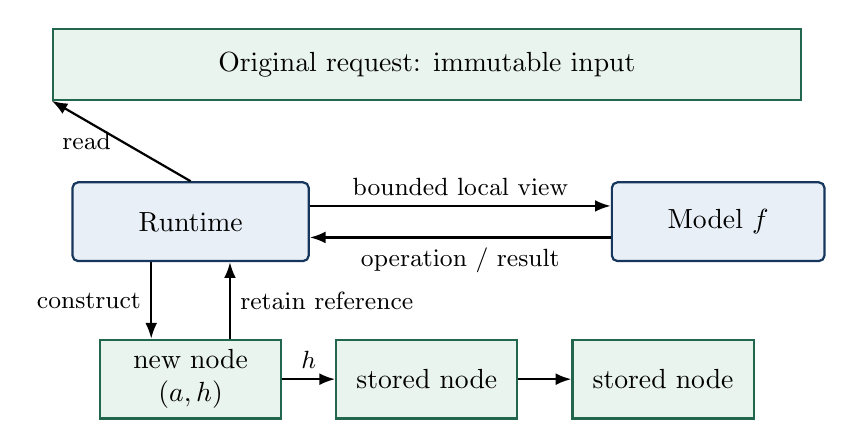
\begin{tikzpicture}[x=10mm,y=10mm]
\node[memory,minimum width=95mm,minimum height=9mm] (input) at (0,2)
 {Original request: immutable input};
\node[module,minimum width=30mm] (rt) at (-3,0) {Runtime};
\node[module,minimum width=27mm] (model) at (3.7,0) {Model $f$};
\node[memory,minimum width=23mm,minimum height=10mm] (new) at (-3,-2)
 {new node\\$(a,h)$};
\node[memory,minimum width=23mm,minimum height=10mm] (old) at (0,-2)
 {stored node};
\node[memory,minimum width=23mm,minimum height=10mm] (end) at (3,-2)
 {stored node};
\draw[flow] (rt.north)--node[left,info]{read}(input.south west);
\draw[flow] ([yshift=2mm]rt.east)--node[above,info]{bounded local view}([yshift=2mm]model.west);
\draw[flow] ([yshift=-2mm]model.west)--node[below,info]{operation / result}([yshift=-2mm]rt.east);
\draw[flow] ([xshift=-5mm]rt.south)--node[left,info]{construct}([xshift=-5mm]new.north);
\draw[flow] ([xshift=5mm]new.north)--node[right,info]{retain reference}([xshift=5mm]rt.south);
\draw[flow] (new.east)--node[above,info]{$h$}(old.west);
\draw[flow] (old.east)--(end.west);
\end{tikzpicture}
\caption{Data construction adds objects that did not occur in the input.
The model handles bounded symbols and operation choices; the runtime stores
nodes and references. A returned reference can denote a large intermediate
answer. Accessing that answer is part of the runtime interface.}
\label{fig:constructed-data}
\end{figure}

Immutable lists can represent two independently accessible stacks. Pushing
$a$ onto a stack with reference $h$ returns $\mathtt{cons}(a,h)$; popping
returns $\mathtt{tail}(h)$ and reads $\mathtt{head}(h)$. The current stack
reference changes, while old nodes remain immutable. This observation
connects data construction directly to the tape simulation.

\subsection{Two stacks provide a read--write tape}

Two independently accessible stacks suffice to implement a tape. Store
the current tape symbol in finite control. The left stack stores symbols
strictly to the left of the head, with the nearest symbol on top; the right
stack stores symbols strictly to the right, again nearest first.
After writing $a'$ in the current cell, a right move performs
\begin{equation}
 \operatorname{push}(L,a'),\qquad
 a\leftarrow\operatorname{pop}(R),
 \label{eq:two-stack-right}
\end{equation}
where popping an empty stack supplies a blank without removing its bottom
marker. A left move swaps $L$ and $R$ in this rule.

\begin{figure}[htbp]
\centering
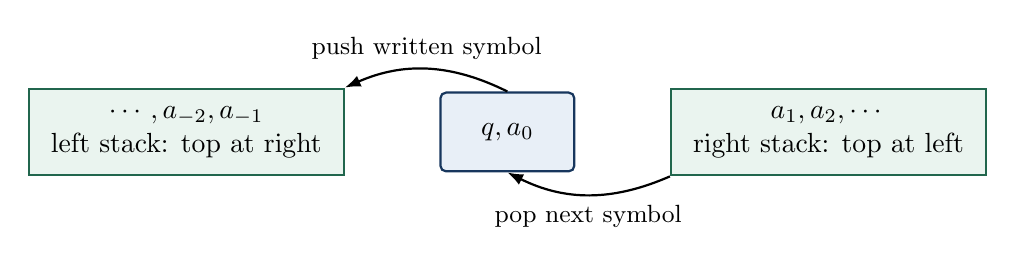
\begin{tikzpicture}[node distance=12mm]
\node[memory,minimum width=40mm,minimum height=11mm] (left) {$\cdots,a_{-2},a_{-1}$\\left stack: top at right};
\node[module,minimum width=17mm,right=of left] (head) {$q,a_0$};
\node[memory,minimum width=40mm,minimum height=11mm,right=of head] (right) {$a_1,a_2,\cdots$\\right stack: top at left};
\draw[flow] (head.north) to[bend right=25] node[above,info]{push written symbol} (left.north east);
\draw[flow] (right.south west) to[bend left=25] node[below,info]{pop next symbol} (head.south);
\end{tikzpicture}
\caption{A rightward tape move using two stacks. Access is still local,
but the two independent stack tops allow movement in both directions.}
\label{fig:two-stacks}
\end{figure}

\begin{proposition}[Two-stack simulation]
\label{prop:two-stacks}
A fixed finite controller with two unbounded stacks can simulate any
fixed Turing machine. Each tape transition uses a bounded number of stack
operations. A run of $T$ transitions visiting $S$ cells uses $O(T)$
stack operations after initialization and $O(S+|x|)$ stored tape symbols
on input $x$. If $S$ includes all initial input cells, the storage bound
is $O(S)$.
\end{proposition}
\begin{proof}
Initialize the two stacks and current symbol from the input. The invariant
is that the two stacks contain the portions of the tape on either side of
the current head, in the orders just described. Writing changes only the
current symbol; \eqref{eq:two-stack-right} and its leftward counterpart
preserve the invariant after movement. The finite transition rule updates
$q$. Each step uses a constant number of operations, and the represented
tape segment contains only visited cells and the initial input.
\end{proof}

The storage bound counts live stack symbols. To attain it with immutable
lists, use an iterative driver or eliminate tail calls, retain only the
current stack roots, and reclaim unreachable nodes. Retaining all earlier
roots in suspended calls or keeping obsolete nodes can instead use
$O(T+|x|)$ storage.

A \emph{scratchpad} here means external writable storage that the runtime
can revisit through a specified interface. A tape, two stacks, and an
addressable store offer different implementations and access costs. The
two-stack construction makes precise how additional memory access can
remove the single-stack restriction. No individual model call needs to
name an arbitrarily large numerical address.

\subsection{Three natural universal implementations}

\begin{corollary}[General computation with constructible lists]
\label{cor:constructible-universal}
First-order recursive programs with finite-symbol list construction and
inspection can simulate every Turing-computable string transformation,
with a write-only output stream for emitted answers.
\end{corollary}
\begin{proof}
The list operations implement two stacks. Apply \cref{prop:two-stacks} to
a machine computing the transformation, using tail-recursive calls for
successive machine steps. Emit the simulated output symbols in order.
\end{proof}

The statement concerns the repertoire of executable programs. A particular
model must still reliably choose or implement the relevant program. Three
common arrangements supply the necessary general execution mechanism:
\begin{enumerate}[leftmargin=*]
\item A recursive runtime with \emph{constructible data} stores lists or
trees and gives the model bounded views and local construction operations.
The preceding proof establishes its computational capacity.
\item A \emph{program executor} runs a stored program with loops or general
recursion and growing data storage. An idealized Python-like interpreter
is an example. The model can produce the program and can remain available
for semantic subcomputations during execution.
\item A \emph{term evaluator} stores and reduces expressions in a universal
language. Untyped lambda calculus, whose expressions represent functions
and function applications, is one example under normal-order evaluation,
which reduces the leftmost outermost available function application.
Growing terms provide computational state. A typed language or restricted
operator library requires its own expressivity analysis.
\end{enumerate}
All three arrangements can use generic software. The runtime need not
contain chess rules, document-specific knowledge, or a task-specific
decomposition algorithm. Such information can come from the input and
from computations the model performs reliably.

For example, write
$\operatorname{Exec}:\Sigma^*\times\Sigma^*\rightharpoonup\Sigma^*$ for a
fixed program executor. A sufficient extension assumption is that a
protocol using trusted model calls produces a stored program $P_x$ with
\begin{equation}
 \operatorname{Exec}(P_x,x)=F(x)\qquad\text{for every }x\in E.
 \label{eq:program-extension}
\end{equation}
The resulting system solves $F$ on $E$, and the executor can use time,
memory, and output length far beyond one model call. The protocol may need
many bounded calls to construct $P_x$; the entire original request $x$
remains external data for the executor. Uniform correctness in
\eqref{eq:program-extension} is a substantive competence assumption.
Correct direct answers on a finite set of short examples do not imply it.

Moving synthesis into software can be useful for precisely this reason.
If synthesis only applies fixed functions to bounded values, the change
can remain within the read-only class. If synthesis constructs new objects
or executes general programs, the tool contributes those capabilities.
Treating arbitrary synthesis as mechanistic is therefore not a
power-preserving change unless its operations are restricted.

\subsection{What the progression establishes}

The comparisons now distinguish a memory extension that improves efficiency
from one that changes which tasks are computable through the interface.
The following statements concern the specified architecture families;
their upper bounds apply to every model operating within those restrictions.
\begin{center}
\small
\renewcommand{\arraystretch}{1.2}
\begin{tabular}{p{0.43\textwidth}p{0.49\textwidth}}
\toprule
Runtime interface & Established consequence \\
\midrule
One-way input and one stack of bounded frames & Context-free upper bound;
cannot decide $L_3$ \\
First-order read-only recursion with saved input references & Exactly
$\mathsf P$ over the permitted finite programs; uncached evaluation can
repeat work exponentially often \\
The same programs with a transparent result cache & Same returned
functions; polynomial evaluation of terminating decision programs \\
General recursion with constructible lists & Universal computation;
the program may use growing time and storage \\
\bottomrule
\end{tabular}
\end{center}

A long output deserves its own accounting. With a write-only output
stream, a slow recursive program can emit exponentially many symbols
without storing them all. The polynomial decision-task characterization
does not bound such an output's length. Applying memoization to a program
that emits symbols is not the pure-call transformation proved in
\cref{lem:memoized}: replaying a cached call must also reproduce its output.
If a long answer is stored and later inspected, the storage and inspection
operations belong to the runtime's data interface.

The remaining model-specific question is which useful tasks admit an
executable decomposition or program using the trusted local repertoire.
The architectural bounds rule out some ambitions even under perfect local
competence. The universal constructions remove that obstruction while
leaving interpretation, decomposition, and correct control as substantive
requirements for the model. The optional constraint example next examines
one concrete family where a local competence assumption gives a positive
extension theorem and an explicit cost for reusable intermediate answers.

\section{Optional reading: constraint combination}
\label{sec:constraints}

This optional example solves a specific version of the extension problem
and examines what a reusable intermediate answer must preserve. The aim is to
decide whether many locally described requirements can hold simultaneously.
Local requirements may come from specifications, program fragments, or
pieces of a structured reasoning task. Even when every local analysis is
correct, independently feasible pieces may be incompatible. A recursive
runtime needs answers that support subsequent combinations.

The construction first specifies the
required information, then proves that finitely many kinds of trusted calls
extend to arbitrarily large expressions. Its limitation quantifies when
bounded summaries cease to suffice.

\subsection{What the parent needs to know}

Consider two subproblems that interact only through a Boolean variable
$z$. One requires $z=0$, and the other requires $z=1$. Each subproblem is
feasible, yet their conjunction is infeasible. Two ``yes'' answers cannot
support correct synthesis.

For a subproblem with internal variables $u$ and shared variables $z$, the
appropriate answer is its \emph{feasibility relation}
\begin{equation}
 A=\{z:\exists u\text{ satisfying the subproblem's constraints}\}.
 \label{eq:boundary-relation}
\end{equation}
The shared variables form the subproblem's \emph{interface}. Internal
variables are removed from the answer, but their effect on possible
interface values is retained. For the two subproblems above,
$A=\{0\}$ and $B=\{1\}$. Joint feasibility is determined by
\begin{equation}
 A\cap B\ne\varnothing.
 \label{eq:intersection-feasible}
\end{equation}
The final answer may be one bit, while a useful intermediate answer is a
set of possible values.

\begin{figure}[htbp]
\centering
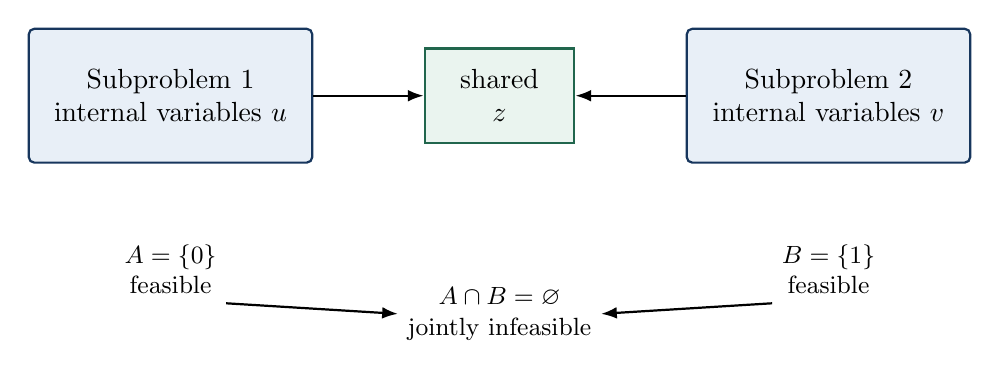
\begin{tikzpicture}[node distance=14mm]
\node[module,minimum width=36mm,minimum height=17mm] (a) {Subproblem 1\\internal variables $u$};
\node[memory,minimum width=19mm,minimum height=12mm,right=of a] (z) {shared\\$z$};
\node[module,minimum width=36mm,minimum height=17mm,right=of z] (b) {Subproblem 2\\internal variables $v$};
\draw[flow] (a)--(z);\draw[flow] (b)--(z);
\node[info,below=9mm of a] (as) {$A=\{0\}$\\feasible};
\node[info,below=9mm of b] (bs) {$B=\{1\}$\\feasible};
\node[info,below=17mm of z] (c) {$A\cap B=\varnothing$\\jointly infeasible};
\draw[flow] (as.south east)--(c.west);
\draw[flow] (bs.south west)--(c.east);
\end{tikzpicture}
\caption{A parent needs the possible values of shared variables. Reporting
only that each child has some solution removes the compatibility information.}
\label{fig:constraints}
\end{figure}

\subsection{A fixed task and its finite trusted set}

To avoid assuming an unspecified decomposition algorithm, take the input
to be an expression describing how constraint modules are combined. Fix
$k\geq1$ Boolean interface positions and let
$Z_k=\{0,1\}^k$. A module denotes a relation $A\subseteq Z_k$.
Write $\tau(A)\in\{0,1\}^{2^k}$ for its membership table in a fixed
lexicographic order. Unused interface positions are permitted; a relation
then does not depend on those coordinates.

The leaves come from a finite vocabulary of bounded descriptions $d$, each
with a specified relation $A_d$. Interpreting $d$ may be a substantial local
task. The vocabulary also contains explicit table leaves $\tab(v)$ for
every $v\in\{0,1\}^{2^k}$. The relation of $\tab(v)$ is $\tau^{-1}(v)$.
These leaves are ordinary input descriptions of a relation,
with a direct, unambiguous meaning. Internal nodes use the following
finite collection of operations:
\begin{align}
 \operatorname{AND}(A,B)&=A\cap B, &
 \operatorname{OR}(A,B)&=A\cup B,\\
 H_i(A)&=\{z\in Z_k:\exists b\in\{0,1\},\ z^{i\leftarrow b}\in A\},
 &&i\in[k].
 \label{eq:relation-operations}
\end{align}
Here $z^{i\leftarrow b}$ replaces coordinate $i$ of $z$ by $b$.
The operation $H_i$ hides an internal Boolean choice: afterward, the answer
no longer depends on the value supplied at interface position $i$.
One may also allow any permutation of the $k$ positions to align the
interfaces of two modules. For a permutation $\pi$ of $[k]$, define
\begin{equation}
 \Pi_\pi(A)=\{z\in Z_k:(z_{\pi(1)},\ldots,z_{\pi(k)})\in A\}.
 \label{eq:permute-relation}
\end{equation}
Since $k$ is fixed, the instruction vocabulary
remains finite. The input supplies these alignments explicitly.

Let $\cT_k$ be the set of finite expressions built from these leaves and
operations, and let $\cA(t)\subseteq Z_k$ denote the relation of expression
$t$. The semantics is defined recursively by
\eqref{eq:relation-operations}. For example,
\begin{equation}
 \cA(\operatorname{AND}(t_1,t_2))=\cA(t_1)\cap\cA(t_2).
 \label{eq:target-relation}
\end{equation}
The string-valued target and the feasibility decision are
\begin{equation}
 F_k(\enc(t))=\tau(\cA(t)),\qquad
 \sat(t)=\I\{\cA(t)\ne\varnothing\}.
 \label{eq:encoded-target}
\end{equation}
Here $\enc$ is a fixed parenthesized encoding. We omit $\enc$ in model
requests when the expression is displayed explicitly.
Forgetting all interface positions produces the full relation for a
feasible module and the empty relation for an infeasible one.

Hiding is local to a subtree. For $k=1$, let $d_0$ require $z=0$ and $d_1$
require $z=1$. Then
\begin{equation}
 \cA(\operatorname{AND}(H_1(d_0),H_1(d_1)))=Z_1,\qquad
 \cA(H_1(\operatorname{AND}(d_0,d_1)))=\varnothing.
 \label{eq:hiding-scope}
\end{equation}
The first expression permits an independent internal choice in each child;
the second requires one shared choice before hiding it. Consequently a
large expression can describe many distinct internal variables while
exposing only $k$ interface positions at any node. The fixed interface
does not restrict the entire problem to $k$ global variables.

Define $W_k$ to contain every leaf and every expression consisting of one
operation applied to table leaves. Examples of trusted requests are
\begin{equation}
 d,\qquad \operatorname{AND}(\tab(\tau(A)),\tab(\tau(B))),\qquad
 H_i(\tab(\tau(A))).
 \label{eq:trusted-examples}
\end{equation}
Because $k$ and the description vocabulary are fixed, $W_k$ is finite.
If the longest original leaf description has length $d_{\max}$, request and
answer lengths satisfy
\begin{equation}
 \max_{w\in W_k}|w|=O(d_{\max}+2^k+k\log(k+1)),
 \qquad |F_k(w)|=2^k.
 \label{eq:relation-call-size}
\end{equation}
The permutation term can be omitted when permutations are absent.
The local competence premise is exactly
\begin{equation}
 f(w)=F_k(w)\qquad(w\in W_k).
 \label{eq:relation-competence}
\end{equation}
Thus the construction uses the original extension formulation: the small
calls and the large input have the same target semantics. The specification
asks for interface relations, not merely isolated feasibility bits. A
model known only to answer yes/no feasibility questions has not been assumed
to supply these richer answers.

\subsection{The extension theorem and its cost}

The runtime evaluates children first, wraps each returned table as a table
leaf, and submits the resulting one-operation expression to the model.
Constructing these requests requires parsing, copying, and stack operations;
the runtime does not interpret the original leaf descriptions or compute
the relation operations itself.

\begin{theorem}[Extension by bounded interface relations]
\label{thm:relation-extension}
Fix $k$, the finite description vocabulary, and $W_k$ as above. There is
one depth-first runtime $R_{\mathrm{tree}}$ such that every model satisfying
\eqref{eq:relation-competence} obeys
\begin{equation}
 R_{\mathrm{tree}}^f(\enc(t))=F_k(\enc(t))\qquad(t\in\cT_k),
 \label{eq:relation-extension}
\end{equation}
and every request belongs to $W_k$. On a tree with $N$ nodes and height
$h$, the runtime uses exactly $N$ model calls, requests of the bounded
length in \eqref{eq:relation-call-size}, and
$O(h(2^k+k\log(k+1)+1))$ stack bits. The input can be read once from a
serialized stream; its storage is separate from the stack bound.
\end{theorem}
\begin{proof}
At a leaf the submitted request is in $W_k$, so the returned table is
correct. At an internal node, the inductively correct child tables are
wrapped as table leaves. The constructed one-operation request belongs to
$W_k$ by definition, and replacing children by tables preserves their
relations. Consequently the model's answer equals the membership table of
the original parent's relation. Induction gives \eqref{eq:relation-extension}.
There is one call at each node. A suspended frame contains an operation,
a finite phase, and at most one completed child table. There are at most
$h$ such frames.
\end{proof}

The conclusion is an unbounded extension in expression size: $k$ and the
model-call budgets stay fixed while $N$ and $h$ can grow. Both total
computation and total stored stack state can exceed the corresponding
resources of one call. For fixed $k$, generic request construction and
copying cost $O(N)$ operations with a constant depending on the fixed
local representation. If implemented directly by table operations, the
relation computations take $O(N2^k)$ elementary Boolean operations for the
AND, OR, and hiding operations. Counting model calls alone leaves the cost
of each model call explicit.

The input organization is a real premise. For a collection of constraints
without a supplied expression, finding a decomposition with small
interfaces is an additional problem. A small interface also does not make
an arbitrary local description easy to interpret; correctness of those
local interpretations remains part of \eqref{eq:relation-competence}.
The theorem isolates how already available local capability can compose.

\begin{example}[A complete evaluation with one shared variable]
\label{ex:one-port}
Take $k=1$ and write tables in the order $0,1$. Let descriptions
$d_0,d_1$ mean $z=0$ and $z=1$, respectively. The trusted leaf calls return
$F_1(d_0)=10$ and $F_1(d_1)=01$. On
$t=\operatorname{AND}(d_0,d_1)$, the runtime makes these two calls and then
submits $\operatorname{AND}(\tab(10),\tab(01))$. The third call returns
$00$, proving infeasibility. On
$\operatorname{OR}(d_0,d_1)$, the corresponding synthesis returns $11$.
Hiding the variable in either single constraint also gives $11$, because
each single constraint has a satisfying choice of $z$.
\end{example}

\Needspace{7\baselineskip}
\begin{example}[A long chain with a fixed-size interface]
\label{ex:constraint-chain}
Let $L\geq1$, let $z_0,\ldots,z_L$ be Boolean variables, and let a local requirement
$C_i\subseteq\{0,1\}^2$ restrict the adjacent pair $(z_{i-1},z_i)$.
The task is to determine whether
\begin{equation}
 \exists z_0,\ldots,z_L\quad
 (z_{i-1},z_i)\in C_i\quad\text{for every }i=1,\ldots,L.
 \label{eq:chain-feasibility}
\end{equation}
A segment can return the relation between its two endpoint variables after
eliminating all variables inside the segment. To combine two segments with
endpoint relations $A,B$, the parent computes
\begin{equation}
 C=\{(u,w):\exists v,\ (u,v)\in A\text{ and }(v,w)\in B\}.
 \label{eq:chain-combine}
\end{equation}
Represent every segment's endpoints in positions 1 and 3, with position 2
unused. Before combining, swap positions 2 and 3 in the left table, and
positions 1 and 2 in the right table. The two tables now constrain
the interface pairs $(u,v)$ and $(v,w)$, respectively. Apply AND and then $H_2$.
The result again has endpoints in positions 1 and 3, so the same procedure
can be used at the next level. Three positions suffice at every combination, while
the number $L+1$ of distinct variables is unbounded.

The runtime receives an expression that splits the chain into adjacent
segments. Model calls interpret each short requirement and combine
returned relations using \eqref{eq:chain-combine}. After expressing each
combination by a fixed number of the allowed operations, the runtime uses
$O(L)$ calls with $k=3$ and tables of eight bits, including unused
positions. A balanced decomposition has height $O(\log(L+1))$, so its
stack uses $O(\log(L+1))$ bits with the fixed local budgets. The example
shows how the extension theorem solves a global consistency problem whose
input and number of internal variables exceed one call's limits.
\end{example}

\subsection{A sharp limit on summaries}

The relation tables might appear to be a wasteful representation. For the
general compatibility question, their worst-case length is unavoidable if
a completed subproblem can communicate only one summary and cannot be
revisited.

\begin{theorem}[Information required by an exact compatibility summary]
\label{thm:summary-lower}
Let every relation $A\subseteq Z_k$ be a possible subproblem. Suppose a
summary map $q:2^{Z_k}\to\{0,1\}^b$ permits exact determination of
$A\cap B\ne\varnothing$ from $q(A)$ and an arbitrary other relation
$B\subseteq Z_k$. Then
\begin{equation}
 b\geq 2^k.
 \label{eq:summary-lower}
\end{equation}
The full membership table attains this bound.
\end{theorem}
\begin{proof}
If $A\ne A'$, choose $z$ in their symmetric difference and set $B=\{z\}$.
Exactly one of $A\cap B$ and $A'\cap B$ is nonempty. Hence a correct
summary must distinguish all $2^{2^k}$ possible relations. Since a
$b$-bit summary has at most $2^b$ values,
$2^b\geq2^{2^k}$, giving \eqref{eq:summary-lower}. A membership table
records exactly one bit for each of the $2^k$ assignments.
\end{proof}

The lower bound concerns information crossing a particular decomposition
boundary. It is not a running-time lower bound for every algorithm for
constraints. A different decomposition can condition on each interface
assignment and use
\[
 \I\{A\cap B\ne\varnothing\}
 =\bigvee_{z\in Z_k}\bigl(\I\{z\in A\}\land\I\{z\in B\}\bigr).
\]
Each conditional answer is one bit; enumeration considers $2^k$ cases.
The conditional subproblems may need further decomposition, and their
model requests must belong to a suitable trusted set. Preparing those
requests and retaining or revisiting the subproblems also count as runtime
operations. Thus the theorem limits a single reusable summary, without
ruling out small answers obtained through repeated conditional computation.
Restricting the possible relations to a family with compact representations
is another way to reduce the summary requirement.

If a returned message is limited to $m$ bits, arbitrary relations on $k$
shared Boolean variables require $2^k\leq m$, or
$k\leq\lfloor\log_2 m\rfloor$. This quantifies a limitation of recursive
decomposition even when the final decision is only one bit. The generic
runtime extends competence to unboundedly many pieces at fixed interface
size, but cannot keep the same message budget while supporting every
larger interface.

\subsection{What the example contributes to the system question}

The problem solved in this section is exact composition of locally
interpreted constraints. The positive result gives a finite trusted request
set, one generic runtime, and an infinite family of larger instances solved
by that runtime. The negative result identifies how much information a
return value must carry when future combinations are unrestricted.

For an AI system, local analyses of requirements or program fragments may
be reliable while their independent short conclusions are insufficient to
construct a globally compatible answer. The relevant mathematical question
is whether the returned objects preserve the dependencies between pieces.
The constraint example supplies an exact answer for one family. It does
not assert that arbitrary natural-language tasks already have the supplied
decomposition or the specified local competence.

A runtime with additional writable memory offers another possibility:
keep intermediate objects and let later computation inspect them through
bounded operations. Such a system can avoid requiring every subproblem to
be compressed once and for all into a short return value. The two-stack
construction shows that bounded local interactions with external memory
can sustain general computation. Which interactions exploit a given model's
substantive skills efficiently remains a task-dependent extension problem.

\section{Optional reading: a queue as a universal interface}
\label{sec:queue}

A \emph{queue} permits deletion at the front and insertion at the rear.
This access rule fits a string transformation especially closely. Fix a
finite alphabet and, for each symbol $a$, a finite production string $v_a$.
The runtime repeatedly applies
\begin{equation}
 Q=abu\longmapsto uv_a,
 \label{eq:tag}
\end{equation}
stopping if fewer than two symbols remain. Reading $a,b$, deleting them,
and appending the bounded production are the runtime's operations. The
model's local task is to return $v_a$ from a bounded request. Such a
computation is called a \emph{2-tag system}.

There exist fixed 2-tag systems that simulate universal Turing computation.
Thus a suitable finite local rule and one unbounded queue suffice for
universality. The tag simulation is a classical existence result; it does
not assert that an arbitrary model's trusted answers supply those rules.
The advancing window in \eqref{eq:advancing-window} provides a related queue
interface, consuming one symbol per step. With exactly one symbol appended,
the queue length stays fixed at the initial input length. Appending two
symbols on some steps allows the queue to grow. In both interfaces, old
symbols remain available at the queue's front until consumed; a fixed
suffix window discards that access.

The memory lesson is now more specific than the statement that long tasks
need memory. A stack is already unbounded memory. The distinction is which
parts of that memory can be accessed while other information is retained.
For a fixed local competence set, additional memory operations can make
new algorithms executable; their usefulness still depends on the task's
structure and the local operations the model performs correctly.

\section{Optional reading: quantitative transformer simulations}
\label{sec:optional}

The tape and queue examples separate a local rule from memory access.
Transformer simulation theorems ask whether a specified attention
architecture can implement the needed access and local computation, and at
what cost. The following results were omitted from class for time. They
provide quantitative upper bounds for constructed simulators.

\begin{theorem}[Fixed-precision simulation bounds; stated without proof]
\label{thm:transformer-simulation}
Fix a Turing machine whose computations on inputs of length $\ell$ have
nondecreasing time and space bounds $T(\ell)$ and $S(\ell)$, in the regime
$T(\ell),S(\ell)\geq\ell$.
\begin{enumerate}[label=(\roman*),leftmargin=*]
\item There is a transformer simulation with a fixed number of parameters
and fixed numerical precision, an $O(S(\ell))$ context window, and
$O(T(\ell)S(\ell))$ generated tokens. Its hard-attention construction
uses relative positions configured to the window length.
\item For every fixed $\varepsilon>0$, a construction for a fixed multitape
machine uses an $O(S(\ell))$ window and
$O(T(\ell)S(\ell)^\varepsilon)$ generated tokens. Model resources may
depend on the machine and $\varepsilon$, but remain constant as $\ell$
grows. Its sparse hard attention uses specified relative offsets depending
on the window length.
\end{enumerate}
\end{theorem}

These bounds distinguish model size and precision from the amount of
accessible context. The positional mechanism is an essential part of the
construction: the first construction explicitly changes a relative-offset
selector when the window grows. The theorem does not claim that every
ordinary fixed-parameter softmax transformer implements the required
addressing rule. Generated-token counts also differ from the arithmetic
cost of evaluating dense attention over a growing context.

Hard attention can select a unique winner using finitely many score values;
for example, scores $1,0,\ldots,0$ yield an exact one-hot selection. Growing
precision is not inherently required for that operation. Identifying the
intended location and implementing the selection are nevertheless substantive
architectural assumptions. Replacing selection by softmax is a different
operation. If $L\geq2$ real-valued logits $s_1,\ldots,s_L$ have spread at most
$\Delta$, then
\begin{equation}
 \max_i\frac{e^{s_i}}{\sum_{j=1}^L e^{s_j}}
 \leq\frac{e^\Delta}{e^\Delta+L-1}.
 \label{eq:attention-spread}
\end{equation}
To prove the bound, subtract the largest logit; every other exponential is
at least $e^{-\Delta}$. Consequently a weight of at least $1/2$ requires
$\Delta\geq\log(L-1)$. The calculation concerns exact softmax with bounded
logit spread. Floating-point underflow or a different numerical attention
rule needs its own analysis.

The simulation results establish possible resource tradeoffs. They do not
give matching lower bounds on simulation time, or establish that a trained
model implements the constructed simulator. The local-competence extension
problem remains meaningful even after universal representability is known.

\section{Take-home messages}
\label{sec:take-home}
\begin{enumerate}[leftmargin=*]
\item An unrestricted next-token rule can represent any string map after
marking the input boundary. Neural implementation adds architecture,
precision, and execution constraints. Parameter bits, active context,
persistent state, execution time, and output length are distinct resources.
\item Bounded persistent state imposes limitations that more iterations
cannot remove. A growing accessible transcript requires a separate analysis
of the attention and addressing operations.
\item Extending trusted local behavior requires task structure and an
executable call protocol. Correct direct answers alone do not provide
correct analysis, synthesis, or program generation.
\item One-way input and one stack of bounded frames give a context-free
upper bound. Even the fixed instruction $I_3$ must fail on some appended
data string. Saved input references permit additional computations while
keeping each model observation bounded.
\item First-order recursion whose data are bounded values and original
input suffixes decides exactly the polynomial-time languages, ranging over
the permitted finite programs. The limitation holds with unrestricted
execution time; a polynomial-time evaluator proves the upper bound even
when the original execution repeats work exponentially often.
\item A transparent cache evaluates each complete pure call once, using
polynomial time for the read-only decision programs. The cache preserves
the returned function; its key must contain all arguments, including input
references. Cached short prompts alone do not identify recursive subproblems.
\item Generalized chess lies beyond this restricted interface even with
perfect local calls. Constructible lists, general program execution, and
universal term evaluation provide natural ways to support general computation.
These capacities still require the model to supply correct task-specific
interpretation and control.
\item Long outputs and intermediate objects must be counted explicitly.
A large object can remain in the runtime and be accessed through bounded
operations. In the optional constraint example, reusable summaries and
conditioning trade memory against repeated computation.
\end{enumerate}

\clearpage
\printendnotes

\section*{Bibliographical notes}

The exact-real recurrent result in \cref{thm:real-rnn} is the arbitrary-language
consequence of \citet{siegelmann1994}, Theorem 3.1 and Corollary 6.3.
The recurrent architecture uses saturated-linear activations and exact
state. Its weights can encode a whole target-specific family of Boolean
circuits. The string-output extension in Endnote~\ref{en:string-output}
is a consequence of that language-recognition result and recurrent control.

\Citet{dooley2026}, Theorem 3.1, prove the $O(t^4)$ VC-dimension bound used
in \cref{thm:real-transformer}. We use the version with a fixed positional
rule and fixed architectural dimensions. Their Proposition 4.5 also
exhibits a noncomputable language recognized by an exact-real transformer.
These results concern one forward pass. The absence of all-task
representation must not be confused with a proof of Turing-incompleteness
for an autoregressive system.

For bounded lengths, \citet{yun2020} prove universal approximation of
continuous sequence maps with positional encodings. Those approximation
results and exact finite-table representation have different hypotheses.
\Cref{thm:finite-table} gives an elementary finite-table construction with
explicit finite arithmetic, using the Boolean lookup idea from Lecture 14.
Sharper memorization bounds appear in \citet{kajitsuka2025}. In their
next-token setting with bounded, separated token vectors, their construction
can use $\widetilde O(\sqrt N)$ parameters and
$\widetilde O(\sqrt N)$ bits per parameter under the stated dimension
conditions. The resulting $\widetilde O(N)$ total description length is
consistent with the counting lower bound; see their Remark 4.4 and
Appendix F for the precision tradeoff. Parameter savings are not the same
as savings in stored information.

For the programming-language use of \emph{runtime}, the Java Virtual Machine
Specification describes stacks, frames, heap storage, and exceptions
\citep{jvms}; the .NET documentation describes execution support and memory
management provided by its Common Language Runtime \citep{microsoftclr}.
The concrete agent-runtime examples
come from the Claude Code, OpenHands, and Deep Agents documentation
\citep{claudecode,openhandsdocs,deepagentsdocs}. The Deep Agents documentation
uses \emph{agent harness} for the surrounding software. These implementations
illustrate different choices of tools, stored state, and control; the
mathematical results in these notes concern the explicitly specified abstract
runtimes.

For chain-of-thought prompting, see \citet{wei2022}; \citet{kojima2022}
study eliciting intermediate reasoning with a short instruction. The
one-call, marked-answer protocol in \cref{sec:cot} explicitly separates
prompt preparation, autoregressive generation, and mechanical extraction.
The marker and extraction map specify our interface; they are not a claim
that every chain-of-thought implementation uses this exact protocol.

\citet{liu2023automata}, Sections~4--5, study learning finite-state
trajectories with shallow transformers. Their primary positive results use
state supervision and report the best of 20 training replicates; training
can be unstable. Figures~6--7 and Appendix~B.2.3--B.2.4 compare distribution
and length generalization with LSTMs and with scratchpad training plus
recency-biased attention. The scratchpad supplies interleaved state labels
during training and predicted states during evaluation, as described in
\cref{sec:cot}. The reported improvements concern the tested parity and
bounded-parenthesis tasks; they are empirical evidence for a particular
training and execution design, not a general guarantee about chain of thought.

The distinction between a finite controller and its external tape continues
the construction in Lecture 14. The finite-state and prefix-collision
arguments are standard automata and streaming-memory arguments. The
single-stack formulation in \cref{thm:stack} is the usual pushdown model.
\citet{alur2005} develop the equivalence between recursive state machines
and pushdown systems; their Theorem 1 provides a formal account of finite
recursive control. Standard pushdown and context-free language results are
also covered in \citet{aho2015}. The two-stack tape simulation is classical.

The read-only language in \cref{def:readonly} is the finite-alphabet version
of the first-order, call-by-value language in \citet{jones2020}, Definition 2.
Token strings are lists, the reference operations are list inspection, and
every bounded local function has a finite case representation. A fixed
binary encoding recovers their Boolean-list formulation. This translation
justifies using the language theorem for the runtime defined in the main text.
Their suffix lemma and polynomial bound on possible calls explain the
argument in \cref{lem:memoized}; their Theorem 2 states the exact
$\mathsf P$ characterization. \Citet{jones2001}, Section 7.3, gives an
explicit caching semantics and proves its equivalence and evaluation-time
bound. Our formulation keeps the model as a trusted bounded local operation
and accounts for the bits needed to retain input references. Neither the
classical characterization nor the cache supplies an algorithm for finding
a suitable decomposition for an arbitrary natural-language request.

\Citet{fraenkel1981} prove the generalized-chess result in \cref{thm:chess}.
Their family has one king per side on an $m\times m$ board, ordinary piece
movements, and populations of the other relevant pieces growing as fixed
positive powers of $m$. The input is an arbitrary position. The notes use
its full board encoding, so its length is polynomial in $m$. The strict
inclusion $\mathsf P\subsetneq\mathsf{EXPTIME}$ follows from the deterministic
time hierarchy theorem; it is distinct from the unresolved separations
involving $\mathsf{NP}$ or $\mathsf{PSPACE}$. The chess reduction itself is
not reproduced here.

Universal tag systems are a classical alternative to direct tape simulation.
\citet{woods2006} study their simulation cost and establish polynomial-time
simulation, improving earlier exponential overheads. The extended
autoregressive system of \citet{schuurmans2024} uses a related queue-like
Lag-system interface. Their Section 2 gives the advancing-window convention
in \eqref{eq:advancing-window} and its extension to block outputs. With a
two-symbol context, suitable rules emitting one symbol simulate deterministic
linear bounded automata; allowing one or two output symbols suffices to simulate
Turing machines. The extra output symbol permits growth of the live queue.
These constructions use the retained queue, not just a fixed suffix.

Several proposed LLM systems can be compared through these interfaces.
PENCIL \citep{pencil2025} removes completed intermediate computations from
the generated context. It addresses retained active state; that state can
still grow with the simulated computation's space. Its simulator theorem
does not establish fixed-context correctness for an arbitrary model.
Recursive Language Models \citep{rlm2025} place the prompt in a Python
execution environment, where generated code can inspect input, create
intermediate objects, and invoke models. The full environment belongs with
general program execution, rather than the restricted read-only language.
Its empirical performance is separate from that architectural capacity.

The $\lambda$-RLM framework of \citet{roy2026}, with several authors from
Huawei Noah's Ark Lab, uses planned recursive decomposition and a fixed
operator library. A model selects a task type and solves bounded leaves;
the runtime supplies task-dependent aggregation. Constructed result lists
and aggregation operators require analysis beyond the cons-free theorem.
Expressing the controller with a fixed-point combinator does not by itself
establish universality of the restricted library. Its stochastic accuracy
bounds are not used in our exact-computation argument.

PAL \citep{gao2023} is a direct example of model-generated programs executed
by an interpreter. BINDER \citep{cheng2023} additionally allows the executed
program to call the model for semantic operations. Decomposed Prompting
\citep{khot2023} makes the decomposer and subtask handlers explicit, with
handlers that can themselves be prompts or symbolic procedures. These
systems illustrate different local competence assumptions; none gives a
general theorem extending arbitrary correct behavior on a finite $W$.

Tree of Thoughts \citep{yao2023} uses model-generated candidates and
evaluations with search over retained reasoning states. Its tree of
alternatives fits the analysis/synthesis description, but the search store
and state representations determine which memory restriction applies.
The memory-augmented construction of \citet{schuurmans2023} instead supplies
an associative read--write store and an explicit finite instruction
repertoire for universal-machine simulation. The repertoire is sufficient
for that simulation, while interpretation of unrestricted instructions
remains a separate requirement.

The constraint construction specializes classical dynamic programming over
decompositions: intermediate results record assignments on the shared
variables. \citet{freuder1990} establish the connection between constraint
structure and complexity linear in instance size and exponential in a
width parameter. The expression language and trusted-set formulation in
\cref{thm:relation-extension} are an elementary formulation for these notes.
\citet{dechter1999}, Sections 2.4 and 10, compare elimination, which stores
intermediate relations, with conditioning search, which instantiates
variables and solves the resulting subproblems. That comparison explains
the alternative to reusable summaries described after
\cref{thm:summary-lower}: memory can be traded for repeated computation.
The exact compatibility-summary lower bound is the direct
distinguishability argument in \cref{thm:summary-lower}; no novelty claim
is intended. \citet{kozen1992} give an elementary exposition and historical
attribution of the tree Myhill--Nerode theorem used in
\appendixref{app:trees}.

The two bounds in \cref{thm:transformer-simulation} are due to
\citet{liwang2025a,liwang2025b}. Remark 4 of the first paper explicitly
identifies the change to relative positional encoding as the context
window changes. The second paper obtains the exponent $6r/K$ for an
$r$-tape machine and a head--layer product $K$; taking sufficiently large
constant model resources yields the stated fixed-$\varepsilon$ form.
\citet{nowak2026} analyze finite-precision causal transformers under
specified numerical semantics. Their finite-state account for no-position
architectures uses accumulators for every possible query, illustrating why
fixed precision and attention implementation must be considered together.

\section*{Glossary}
\begin{description}[style=nextline,leftmargin=1.5em,labelindent=0pt]
\item[Control token]
A distinguished element of the token alphabet $\Sigma$ to which the runtime
assigns an operation. The generation runtime interprets $\eos$ as ending
the current model call.
\item[Model call $f$]
A string-to-string computation. In the autoregressive construction,
$f=G^p$: a generation runtime $G$ repeatedly invokes the next-token model
$p$. Trusted calls terminate with their specified answers.
\item[Chain-of-thought protocol]
The runtime prepares a prompt with $J$, generates reasoning and a marked
answer with $f$, and returns the answer through $E$: $R_{\mathrm{CoT}}^f=E\circ f\circ J$.
Generated length and returned-answer length are separate resources.
\item[Next-token rule and kernel]
A deterministic rule $p$ chooses one token from a prefix. A probabilistic
kernel $\pi(\cdot\mid h)$ assigns a next-token distribution to each prefix
$h$; a fixed decoding convention turns the kernel into a rule.
\item[Exact-real and fixed-precision models]
Exact-real computation permits arbitrary real weights and exact arithmetic.
Fixed precision restricts stored numerical values to a specified finite set.
\item[Shattering and VC dimension]
A binary function family shatters a set if it realizes every binary
labeling of that set. Its VC dimension is the largest size of such a set.
\item[Runtime system $R$]
The algorithm that prepares and schedules calls, manages state, and returns
the system output. $R^f$ denotes execution with access to model $f$.
\emph{Agent harness} denotes the same surrounding software in these notes.
\item[Fixed suffix and advancing window]
A fixed suffix gives the model the most recent $K$ tokens. An advancing
window moves through a retained string while outputs are appended at its end;
the live queue can exceed the active context in length.
\item[Configuration]
All persistent information that can affect future computation, including
controller state, accessible tokens, caches, and usable counters.
\item[Trusted set $W$ and extension set $E_R(F,W)$]
$W$ contains requests on which model correctness is assumed. The extension
set contains inputs solved correctly with termination and queries only in $W$.
\item[Analysis and synthesis]
Analysis supplies subproblems and a combination instruction. Synthesis
combines their answers according to that instruction.
\item[Sound decomposition and compatibility set]
The pair $(A,S)$ is sound for $F$ on $E$ when the synthesis identity holds
for every $x\in E$. The set $\cC_F(A,S)$ contains precisely those inputs.
The identity at all internal nodes, correct direct leaf answers, and
termination together imply recursive correctness.
\item[Synthesis request]
The encoded instruction and child answers submitted for synthesis.
When synthesis is a model call, the whole request must be trusted.
\item[Stack and call frame]
A stack has last-in, first-out access. A call frame stores the information
needed to resume a suspended call. Bounded frames have finitely many possible
values; frames holding input references can require $O(\log(n+2))$ bits.
\item[Decision problem and language]
A yes/no task is identified with the language of strings whose answer is
yes. A decider terminates on every input with its correct yes/no answer.
\item[Finite persistent control]
The information retained outside the explicitly declared stores ranges
over a fixed finite set independent of input length.
\item[Pushdown automaton]
A finite controller with one stack over a finite alphabet and one-way
input, possibly taking transitions without consuming input.
\item[First-order read-only recursion]
Recursive procedures whose values are bounded atoms or original input
suffixes. Functions are not passed as data; calls have no side effects or
access to caller frames. The absence of list construction is called
\emph{cons-free} computation.
\item[Call protocol $P$ and execution $R_P^f$]
A fixed finite program specifying recursive calls, runtime operations, and
bounded model requests. $R_P^f$ is its execution using model $f$; all data
affecting a pure call's result are explicit arguments or fixed constants.
\item[Memoization and complete call key]
Memoization caches a pure call's result under its procedure and complete
argument tuple. A transparent cache changes execution cost without providing
program-visible state. ACTIVE and completed entries distinguish pending
computations from available results.
\item[Polynomial time and EXPTIME]
$\mathsf P$ contains decision problems solvable in $n^{O(1)}$ time;
$\mathsf{EXPTIME}$ uses $2^{n^{O(1)}}$ time. Completeness identifies problems
to which every problem in the class reduces in polynomial time.
\item[Heap and data constructor]
A heap stores allocated objects accessed through references. The constructor
$\mathtt{cons}(a,h)$ creates a list node containing a symbol and a tail
reference; inspection reads the node's fields.
\item[Scratchpad]
External writable state that can be revisited through a specified memory
interface. The term alone does not specify access operations or their cost.
\item[Queue and 2-tag system]
A queue deletes at the front and appends at the rear. A 2-tag system
replaces $abu$ by $uv_a$ for a fixed finite production rule $a\mapsto v_a$.
\item[Interface and feasibility relation]
The interface contains the variables through which a subproblem interacts
with its surroundings. Its feasibility relation records the assignments
that extend to a solution inside the subproblem.
\item[Summary state and enclosing tree]
A summary state is the bounded result passed from a subtree to its parent.
An enclosing tree has one hole where a subtree may be inserted; it specifies
how later computation uses that subtree.
\item[Diagram conventions]
Blue boxes represent computational components; green boxes represent stored
state or returned data. Arrow labels identify the information passed through
an interface. A box's drawn size does not indicate its memory capacity.
\end{description}

\Needspace{32\baselineskip}
\section{Exercises}
\label{sec:exercises}

\exerciseinstructions
\setcounter{courseexercise}{0}
\begin{exercisechunk}
\item \textbf{Every string map has a next-token representation.}
\label[exercise]{ex:l16-autoregressive-representation}
\exerciseprofile{2}{1}{1}{\exproof\quad\exconstruction}{%
Separate the expressiveness of autoregressive output from the difficulty
of representing its next-token rule.}
Let $\Delta$ be a finite data alphabet and
$\Sigma=\Delta\cup\{\mathtt{SEP},\mathtt{EOS}\}$, where the two added
tokens are distinct and do not belong to $\Delta$.
Given $p:\Sigma^*\to\Sigma$, the runtime $G$ starts from
$h_0=x\mathtt{SEP}$, repeatedly appends $p(h)$ to the current prefix,
and stops when $p(h)=\mathtt{EOS}$, without appending the stop token.
It returns only the generated answer, excluding $x\mathtt{SEP}$.

For an arbitrary function $F:\Delta^*\to\Delta^*$, construct a total
next-token rule $p$ and prove that $G^p(x)=F(x)$ for every $x\in\Delta^*$.
Your construction must define $p$ on all strings in $\Sigma^*$ and cover
the case $F(x)$ is empty. Neither $F$ nor $p$ is assumed computable.
\end{exercisechunk}


\appendix
\section{An exact finite-context transformer construction}
\label{app:finite-table}

We prove the upper bound in \cref{thm:finite-table} without hard attention
or an exact-real parameter carrying an unbounded table. Restated, for
$t\geq1$, $q=|\Sigma|\geq2$, and $N_t=\sum_{j=0}^tq^j$, every
$p:\Sigma^{\leq t}\to\Sigma$ has the stated two-block representation
using $O(tqN_t+(tq)^2)$ scalar parameters and $O(\log(t+q))$ bits per
numerical value.

\begin{proof}
Use a padding symbol $\bot$ and a readout symbol outside $\Sigma$.
Right-pad each input $w$ to a string $\bar w$ of length $t$ and then add
padding positions and a final readout position so that the total length is
\[
 M=2^{\lceil\log_2(t+1)\rceil}<2(t+1).
\]
Write $\xi_1,\ldots,\xi_M$ for this full sequence: its first $t$
symbols form $\bar w$, its last symbol is the readout, and any intervening
symbols are padding.
The input embedding concatenates one-hot token and position vectors.
Reserve separate, initially zero coordinates for the intermediate
quantities below. A positional flag $s_i=\I\{i=M\}$ identifies the readout.
Residual branches write into these reserved coordinates and preserve the
input coordinates and flag. No layer normalization is used.

In the first block, set all attention matrices to zero. At position $i$, a
ReLU feed-forward block computes
\[
 r_{j,a}^{(i)}
 =\operatorname{ReLU}\bigl(\I\{i=j\}+\I\{\xi_i=a\}-1\bigr),
 \qquad j\leq t,\quad a\in\Sigma\cup\{\bot\}.
\]
Thus $r_{j,a}^{(i)}$ is one exactly when position $i$ is the input slot $j$
and that slot contains $a$. Each vector has $t(q+1)$ coordinates.

In the second block, use one attention head with key dimension one and
zero queries and keys. At the final readout, all $M$ causal positions are
visible, so every attention weight is $1/M$. Use the $r$ coordinates as
values and multiply the attention output by $M$. The readout therefore
contains
\[
 z_{j,a}^{(M)}=\sum_{i=1}^{M}r_{j,a}^{(i)}=\I\{\bar w_j=a\}.
\]
The vector $z^{(M)}$ identifies the entire padded input exactly. Earlier
positions may use rounded weights $1/i$; those positions are not used as
readouts and are not attended to by any later block. Keeping their
rounded attention weights in $[0,1]$ guarantees
$0\leq z_{j,a}^{(i)}\leq M$.

For each possible input $v\in D_t$, the second feed-forward block has one
hidden unit. Let $C=tM+2$ and define, at each position $i$,
\[
 u_v^{(i)}=\operatorname{ReLU}\left(
   \sum_{j=1}^{t}z_{j,\bar v_j}^{(i)}-(t-1)-C(1-s_i)\right).
\]
At the readout, $s_M=1$, so $u_v^{(M)}=1$ if $v=w$ and is zero otherwise:
distinct padded strings disagree in at least one slot. At any earlier
position, the sum is at most $tM$, and the term $-C$ makes every lookup
unit zero. This gate prevents earlier positions from producing a sum of
exponentially many active lookup units.

The output logits in reserved channels are
\[
 \ell_a^{(i)}=\sum_{v\in D_t:\,p(v)=a}u_v^{(i)}\qquad(a\in\Sigma).
\]
Exactly one final logit is one, namely $\ell_{p(w)}^{(M)}$; the others are
zero. Greedy decoding therefore returns $p(w)$ with no tie.

The hidden dimension is $O(tq)$. The first feed-forward block has
$O(tq)$ hidden units and the second has $N_t$ units. Counting dense
matrices, including zero entries, gives
\[
 P=O\bigl((tq)^2+tqN_t\bigr).
\]
All task-dependent information is in finite lookup weights. The only
noninteger values needed in the exact readout computation are multiples
of $1/M$. Softmax evaluates exponentials only at zero, and its final
normalizing denominator is the power of two $M$. Binary fixed-point
arithmetic with $\log_2 M$ fractional bits therefore represents the final
attention weights exactly. Intermediate magnitudes are polynomial in
$t+q$, including the gate constant $C$; $O(\log(t+q))$ integer, sign,
and fractional bits suffice. Choose enough integer bits to avoid overflow
and round every operation to the nearest representable value, with a fixed
rule for ties. Operations on the readout's computation path are exact.
Earlier-position divisions may be rounded, since their lookup units are
gated off.
\end{proof}

The construction exposes both information and implementation costs. A
large table uses many finite weights. More economical parameter counts
may instead store more bits in each weight; the description-bit lower
bound counts both resources.

\section{Why one stack cannot recognize three equal blocks}
\label{app:pumping}

The single-stack limitation uses a language that requires matching three
consecutive block lengths. We give the standard obstruction so that the
nonuniversality claim does not depend only on a class name.

\begin{lemma}[Pumping property of context-free languages]
\label{lem:cfl-pumping}
For every context-free language $L$, there exists $p\geq1$ such that every
$w\in L$ with $|w|\geq p$ admits a factorization $w=uvxyz$ with
$|vxy|\leq p$, $|vy|\geq1$, and
\begin{equation}
 uv^i xy^i z\in L\qquad\text{for every integer }i\geq0.
 \label{eq:cfl-pumping}
\end{equation}
\end{lemma}

The lemma follows from repetition of a nonterminal on a sufficiently long
path in a context-free grammar's parse tree. The repeated nonterminal permits
the intervening derivation to be removed or repeated. In a binary normal
form, a bound on the number of distinct nonterminals supplies a uniform
$p$. We use the lemma to prove the promised separation.

\begin{proposition}[Restatement of the language obstruction in \cref{thm:stack}]
The language $L_3=\{a^j b^j c^j:j\geq1\}$ is not context-free.
\end{proposition}
\begin{proof}
Suppose the pumping property holds with constant $p$, and take
$w=a^p b^p c^p$. Any substring of length at most $p$ meets at most two of
the three blocks. Thus $vxy$ in the lemma misses at least one symbol type.
Deleting $v$ and $y$ removes at least one symbol and leaves the count of
the missed type equal to $p$. At least one other count is smaller than
$p$, so $uxz\notin L_3$, contradicting \eqref{eq:cfl-pumping} with $i=0$.
\end{proof}

\section{Which tree computations admit bounded summaries?}
\label{app:trees}

The compatibility example asks whether a completed subproblem can be
replaced by a bounded result that supports every later combination. The
same question has an exact answer for a fixed bottom-up tree interface.
The theorem below characterizes the information required by that interface;
it does not characterize every recursive algorithm or runtime with a heap.

Let $\Lambda$ be a finite set of node labels. Each label $a$ has a fixed
arity $r(a)$, its number of children. Such a collection is a
\emph{ranked alphabet}. Let $\cT$ be the finite trees built from these
labels, and let $H:\cT\to\{0,1\}$ be a decision task. A
\emph{bottom-up summary scheme} consists of a finite state set $Q$, maps
\begin{equation}
 \delta_a:Q^{r(a)}\to Q\quad(a\in\Lambda),\qquad
 \rho:Q\to\{0,1\},
 \label{eq:tree-scheme}
\end{equation}
and the recursive summary
$q(a(t_1,\ldots,t_{r(a)}))=\delta_a(q(t_1),\ldots,q(t_{r(a)}))$.
Correctness means $H(t)=\rho(q(t))$ for every tree. At a leaf,
$\delta_a$ has no child arguments. This scheme is also called a
deterministic bottom-up \emph{tree automaton} with an output map.

An \emph{enclosing tree} $C$ has exactly one hole. Write $C[t]$ for the
complete tree obtained by inserting $t$ into that hole; the hole by itself
is also allowed. The word ``context'' is often used for $C$ in automata
theory. Here an enclosing tree describes the use of a subproblem, not the
token context of a model call. Define
\begin{equation}
 u\equiv_H v
 \quad\Longleftrightarrow\quad
 H(C[u])=H(C[v])\text{ for every enclosing tree }C.
 \label{eq:tree-equivalence}
\end{equation}
The equivalence classes describe precisely which distinctions later
computation can require.

\begin{theorem}[Tree Myhill--Nerode characterization]
\label{thm:tree-mn}
There exists a finite bottom-up summary scheme computing $H$ exactly if and only if
$\equiv_H$ has finitely many equivalence classes. When the number of
classes is $M$, the minimum number of reachable summary states is $M$.
\end{theorem}
\begin{proof}
For necessity, suppose $q(u)=q(v)$. Induction upward along the unique path
from the hole of $C$ to its root gives $q(C[u])=q(C[v])$. Therefore
$H(C[u])=H(C[v])$ for every $C$, so $u\equiv_H v$.
Every inequivalent pair must have different states, giving $|Q|\geq M$.

For sufficiency, take $Q$ to be the equivalence classes and set
\begin{equation}
 \delta_a([t_1],\ldots,[t_r])=[a(t_1,\ldots,t_r)].
 \label{eq:quotient-combine}
\end{equation}
The operation is well-defined. Replacing one $t_i$ by an equivalent tree
inside any enclosing tree preserves $H$, by the definition of equivalence.
Replacing children one at a time proves that the class on the right does
not depend on the chosen representatives. Define $\rho([t])=H(t)$; the
enclosing tree consisting of a hole makes this well-defined as well.
Induction on the input tree shows that its computed state is $[t]$.
The scheme therefore computes $H$ with exactly $M$ reachable states.
\end{proof}

The theorem supplies a necessary and sufficient structural condition for
one bounded message per completed subtree. To execute the scheme with an
existing model, its local transition and leaf requests must still be
trusted. The theorem does not infer those abilities from unrelated correct
answers. The theorem also permits a number of states far beyond a practical call
budget; with $b$ available summary bits, one needs $M\leq2^b$.

For the constraint example, two different relations are distinguishable
by conjunction with a singleton relation followed by a feasibility test.
The $2^{2^k}$ possible relations therefore give distinct equivalence
classes for that use of a subproblem. Their membership tables supply
matching summary states. \Cref{thm:summary-lower} is the resulting concrete
state bound, established directly without the general theorem.

\begin{example}[Equality of arbitrary subtrees]
Let $\cU$ be an infinite family of finite trees. Consider the decision
task on a root pair $(u,v)$ that returns $1$ exactly when $u=v$.
If each child is replaced by a state from a fixed finite set, there exist
$u\ne v$ with $q(u)=q(v)$. The root then receives identical state pairs on
$(u,u)$ and $(u,v)$ and cannot answer correctly on both.
Keeping the two trees and comparing corresponding nodes is a different
access protocol. It may use short local comparisons, but the runtime must
retain and traverse both objects. The failure of independent summaries
does not prohibit that computation.
\end{example}

\clearpage
\begin{thebibliography}{99}

\bibitem[Aho(n.d.)]{aho2015}
Alfred V. Aho.
\newblock Pushdown automata and context-free grammars.
\newblock COMS W3261 course materials, Columbia University, undated.
\newblock \url{https://www.cs.columbia.edu/~aho/cs3261/Lectures/L8-PDA.html}.

\bibitem[Alur et~al.(2005)]{alur2005}
Rajeev Alur, Michael Benedikt, Kousha Etessami, Patrice Godefroid,
Thomas Reps, and Mihalis Yannakakis.
\newblock Analysis of recursive state machines.
\newblock \emph{ACM Transactions on Programming Languages and Systems},
27(4):786--818, 2005.
\newblock \url{https://www.cis.upenn.edu/~alur/toplas2005.pdf}.

\bibitem[Anthropic(n.d.)]{claudecode}
Anthropic.
\newblock How Claude Code works.
\newblock Claude Code documentation, accessed October 27, 2026.
\newblock \url{https://code.claude.com/docs/en/how-claude-code-works}.

\bibitem[Cheng et~al.(2023)]{cheng2023}
Zhoujun Cheng, Tianbao Xie, Peng Shi, Chengzu Li, Rahul Nadkarni,
Yushi Hu, Caiming Xiong, Dragomir Radev, Mari Ostendorf,
Luke Zettlemoyer, Noah A. Smith, and Tao Yu.
\newblock Binding language models in symbolic languages.
\newblock \emph{Proceedings of ICLR}, 2023.
\newblock \url{https://arxiv.org/abs/2210.02875}.

\bibitem[Dechter(1999)]{dechter1999}
Rina Dechter.
\newblock Bucket elimination: A unifying framework for reasoning.
\newblock \emph{Artificial Intelligence}, 113:41--85, 1999.
\newblock \url{https://ics.uci.edu/~dechter/publications/r76A.pdf}.

\bibitem[Dooley et~al.(2026)]{dooley2026}
Gavin Dooley, Andy Yang, Yijia Jessica Zhu, David Chiang, Peter Cholak,
and Anand Pillay.
\newblock VC dimension and expressivity of real-valued transformers.
\newblock arXiv:2609.31999, 2026.
\newblock \url{https://arxiv.org/abs/2609.31999}.

\bibitem[Fraenkel and Lichtenstein(1981)]{fraenkel1981}
Aviezri S. Fraenkel and David Lichtenstein.
\newblock Computing a perfect strategy for $n\times n$ chess requires
time exponential in $n$.
\newblock \emph{Journal of Combinatorial Theory, Series A},
31(2):199--214, 1981.
\newblock \url{https://doi.org/10.1016/0097-3165(81)90016-9}.

\bibitem[Freuder(1990)]{freuder1990}
Eugene C. Freuder.
\newblock Complexity of $k$-tree structured constraint satisfaction problems.
\newblock \emph{Proceedings of AAAI}, pages 4--9, 1990.
\newblock \url{https://cdn.aaai.org/AAAI/1990/AAAI90-001.pdf}.

\bibitem[Gao et~al.(2023)]{gao2023}
Luyu Gao, Aman Madaan, Shuyan Zhou, Uri Alon, Pengfei Liu,
Yiming Yang, Jamie Callan, and Graham Neubig.
\newblock PAL: Program-aided language models.
\newblock \emph{Proceedings of ICML}, 2023.
\newblock \url{https://arxiv.org/abs/2211.10435}.

\bibitem[Jones(2001)]{jones2001}
Neil D. Jones.
\newblock The expressive power of higher-order types or, life without CONS.
\newblock \emph{Journal of Functional Programming}, 11(1):55--94, 2001.
\newblock \url{https://doi.org/10.1017/S0956796800003889}.

\bibitem[Jones et~al.(2020)]{jones2020}
Neil D. Jones, Siddharth Bhaskar, Cynthia Kop, and Jakob Grue Simonsen.
\newblock Cons-free programs and complexity classes between LOGSPACE and PTIME.
\newblock arXiv:2008.02932, 2020.
\newblock \url{https://arxiv.org/abs/2008.02932}.

\bibitem[Kajitsuka and Sato(2025)]{kajitsuka2025}
Tokio Kajitsuka and Issei Sato.
\newblock On the optimal memorization capacity of transformers.
\newblock \emph{Proceedings of ICLR}, 2025.
\newblock \url{https://arxiv.org/abs/2409.17677}.

\bibitem[Khot et~al.(2023)]{khot2023}
Tushar Khot, Harsh Trivedi, Matthew Finlayson, Yao Fu,
Kyle Richardson, Peter Clark, and Ashish Sabharwal.
\newblock Decomposed prompting: A modular approach for solving complex tasks.
\newblock \emph{Proceedings of ICLR}, 2023.
\newblock \url{https://arxiv.org/abs/2210.02406}.

\bibitem[Kojima et~al.(2022)]{kojima2022}
Takeshi Kojima, Shixiang~Shane Gu, Machel Reid, Yutaka Matsuo, and Yusuke Iwasawa.
\newblock Large language models are zero-shot reasoners.
\newblock \emph{Advances in Neural Information Processing Systems}, 2022.
\newblock \url{https://arxiv.org/abs/2205.11916}.

\bibitem[Kozen(1992)]{kozen1992}
Dexter Kozen.
\newblock On the Myhill--Nerode theorem for trees.
\newblock \emph{Bulletin of the EATCS}, 47:170--173, 1992.
\newblock \url{https://www.cs.cornell.edu/kozen/Papers/mn.pdf}.

\bibitem[LangChain(n.d.)]{deepagentsdocs}
LangChain.
\newblock Deep Agents overview.
\newblock Documentation, accessed October 27, 2026.
\newblock \url{https://docs.langchain.com/oss/python/deepagents/overview}.

\bibitem[Li and Wang(2025a)]{liwang2025a}
Qian Li and Yuyi Wang.
\newblock Constant bit-size transformers are Turing complete.
\newblock \emph{Advances in Neural Information Processing Systems}, 2025.
\newblock \url{https://arxiv.org/abs/2506.12027}.

\bibitem[Li and Wang(2025b)]{liwang2025b}
Qian Li and Yuyi Wang.
\newblock Efficient Turing machine simulation with transformers.
\newblock arXiv:2512.00003, version 2, 2025.
\newblock \url{https://arxiv.org/abs/2512.00003}.

\bibitem[Liu et al.(2023)]{liu2023automata}
Bingbin Liu, Jordan T. Ash, Surbhi Goel, Akshay Krishnamurthy, and Cyril Zhang.
\newblock Transformers Learn Shortcuts to Automata.
\newblock In \emph{International Conference on Learning Representations}, 2023.
\newblock \url{https://arxiv.org/abs/2210.10749}.

\bibitem[Microsoft(n.d.)]{microsoftclr}
Microsoft.
\newblock Common Language Runtime (CLR) overview.
\newblock .NET documentation, accessed October 27, 2026.
\newblock \url{https://learn.microsoft.com/en-us/dotnet/standard/clr}.

\bibitem[Nowak et~al.(2026)]{nowak2026}
Franz Nowak, Ryan Cotterell, and Reda Boumasmoud.
\newblock A compositional theory of causally masked transformers.
\newblock arXiv:2607.26988, 2026.
\newblock \url{https://arxiv.org/abs/2607.26988}.

\bibitem[OpenHands(n.d.)]{openhandsdocs}
OpenHands.
\newblock Agent: High-level architecture of the reasoning-action loop.
\newblock Documentation, accessed October 27, 2026.
\newblock \url{https://docs.openhands.dev/sdk/arch/agent}.

\bibitem[Oracle(n.d.)]{jvms}
Oracle.
\newblock The structure of the Java Virtual Machine.
\newblock \emph{The Java Virtual Machine Specification, Java SE 21},
Chapter~2, accessed October 27, 2026.
\newblock \url{https://docs.oracle.com/javase/specs/jvms/se21/html/jvms-2.html}.

\bibitem[Roy et~al.(2026)]{roy2026}
Amartya Roy, Rasul Tutunov, Xiaotong Ji, Matthieu Zimmer,
and Haitham Bou-Ammar.
\newblock The $\mathbf Y$-combinator for LLMs: Solving long-context rot
with $\lambda$-calculus.
\newblock arXiv:2603.20105, 2026.
\newblock \url{https://arxiv.org/abs/2603.20105}.

\bibitem[Schuurmans(2023)]{schuurmans2023}
Dale Schuurmans.
\newblock Memory augmented large language models are computationally universal.
\newblock arXiv:2301.04589, 2023.
\newblock \url{https://arxiv.org/abs/2301.04589}.

\bibitem[Schuurmans et~al.(2024)]{schuurmans2024}
Dale Schuurmans, Hanjun Dai, and Francesco Zanini.
\newblock Autoregressive large language models are computationally universal.
\newblock arXiv:2410.03170, 2024.
\newblock \url{https://arxiv.org/abs/2410.03170}.

\bibitem[Siegelmann and Sontag(1994)]{siegelmann1994}
Hava~T. Siegelmann and Eduardo~D. Sontag.
\newblock Analog computation via neural networks.
\newblock \emph{Theoretical Computer Science}, 131(2):331--360, 1994.
\newblock \url{https://www.sontaglab.org/FTPDIR/siegelmann_sontag_tcs1994.pdf}.

\bibitem[Wei et~al.(2022)]{wei2022}
Jason Wei, Xuezhi Wang, Dale Schuurmans, Maarten Bosma, Brian Ichter,
Fei Xia, Ed Chi, Quoc Le, and Denny Zhou.
\newblock Chain-of-thought prompting elicits reasoning in large language models.
\newblock \emph{Advances in Neural Information Processing Systems}, 2022.
\newblock \url{https://arxiv.org/abs/2201.11903}.

\bibitem[Woods and Neary(2006)]{woods2006}
Damien Woods and Turlough Neary.
\newblock On the time complexity of 2-tag systems and small universal Turing
machines.
\newblock \emph{Proceedings of FOCS}, pages 439--446, 2006.
\newblock \url{https://arxiv.org/abs/cs/0612089}.

\bibitem[Yang et~al.(2025)]{pencil2025}
Chenxiao Yang, Nathan Srebro, David McAllester, and Zhiyuan Li.
\newblock PENCIL: Long thoughts with short memory.
\newblock \emph{Proceedings of ICML}, PMLR 267:71092--71156, 2025.
\newblock \url{https://proceedings.mlr.press/v267/yang25ac.html}.

\bibitem[Yao et~al.(2023)]{yao2023}
Shunyu Yao, Dian Yu, Jeffrey Zhao, Izhak Shafran, Thomas~L. Griffiths,
Yuan Cao, and Karthik Narasimhan.
\newblock Tree of Thoughts: Deliberate problem solving with large language models.
\newblock \emph{Advances in Neural Information Processing Systems}, 2023.
\newblock \url{https://arxiv.org/abs/2305.10601}.

\bibitem[Yun et~al.(2020)]{yun2020}
Chulhee Yun, Srinadh Bhojanapalli, Ankit Singh Rawat, Sashank~J. Reddi,
and Sanjiv Kumar.
\newblock Are transformers universal approximators of sequence-to-sequence functions?
\newblock \emph{Proceedings of ICLR}, 2020.
\newblock \url{https://arxiv.org/abs/1912.10077}.

\bibitem[Zhang et~al.(2025)]{rlm2025}
Alex L. Zhang, Tim Kraska, and Omar Khattab.
\newblock Recursive language models.
\newblock arXiv:2512.24601, 2025.
\newblock \url{https://arxiv.org/abs/2512.24601}.

\end{thebibliography}
\end{document}
